% 	TO DO: 
%	Wie passen die neu eingefügten Bilder (RF,fertilty hist)
 

%	MZ Tabelle nicht einfügen: DDRD estimate von Regression mit 3 CG


%--------------------------------------------------------------------
%	DOCUMENT CLASS
%--------------------------------------------------------------------
\documentclass[11pt, a4paper]{article} % type of document (paper, presentation, book,...); scrartcl class with sans serif titles, European layout 
\usepackage{fullpage} % leaves less space at margins of page
\usepackage[onehalfspacing]{setspace} % determine line pitch to 1.5

%--------------------------------------------------------------------
%	INPUT
%--------------------------------------------------------------------
\usepackage[T1]{fontenc} 	% Use 8-bit encoding that has 256 glyphs
\usepackage[utf8]{inputenc} % Required for including letters with accents, Umlaute,...
\usepackage{float} 			% better control over placement of tables and figures in the text
\usepackage{graphicx} 		% input of graphics
\usepackage{xcolor} 		% advanced color package
\usepackage{url, hyperref} 	% include (clickable) URLs
\usepackage{pdfpages}		% insert pages of external pdf documents
\setlength{\parskip}{0em}	% vertical spacing for paragraphs
\setlength{\parindent}{0em}	% horizonzal spacing for paragraphs
\usepackage{tikz}
\usepackage{tikzscale}		% helps to adjust tikz pictures to textwidth/linewidth
\usetikzlibrary{decorations.pathreplacing}
\usetikzlibrary{patterns}
\usetikzlibrary{arrows}

% Have sections in TOC, but not in text
\usepackage{xparse}% for easier management of optional arguments
\ExplSyntaxOn
\NewDocumentCommand{\TODO}{msom}
{
	\IfBooleanF{#1}% do nothing if it's starred
	{
		\cs_if_eq:NNT #1 \chapter { \cleardoublepage\mbox{} }
		\refstepcounter{\cs_to_str:N #1}
		\IfNoValueTF{#3}
		{
			\addcontentsline{toc}{\cs_to_str:N #1}{\protect\numberline{\use:c{the\cs_to_str:N #1}}#4}
		}
		{
			\addcontentsline{toc}{\cs_to_str:N #1}{\protect\numberline{\use:c{the\cs_to_str:N #1}}#3}
		}
	}
	\cs_if_eq:NNF #1 \chapter { \mbox{} }% allow page breaks after sections
}
\ExplSyntaxOff

%--------------------------------------------------------------------
%	TABLES, FIGURES, LISTS
%--------------------------------------------------------------------
\usepackage{booktabs} 		% better tables
\usepackage{longtable}		% tables that may be continued on the next page
\usepackage{threeparttable} % add notes below tables
\renewcommand\TPTrlap{}		% add margins on the side of the notes
	\renewcommand\TPTnoteSettings{%
	\setlength\leftmargin{5 pt}%
	\setlength\rightmargin{5 pt}%
}
\usepackage[
center, format=plain,
font=normalsize,
nooneline,
labelfont={bf}
]{caption} 				% change format of captions of tables and graphs 
%USED IN MPHIL: \usepackage[labelfont=bf,labelsep = period, singlelinecheck=off,justification=raggedright]{caption}, other specifications which are nice: labelformat = parens -> number in paranthesis 


%\usepackage{threeparttablex} % for "ThreePartTable" environment, helps to combine threepart and longtable

% Allow line breaks with \\ in column headings of tables
\newcommand{\clb}[3][c]{%
	\begin{tabular}[#1]{@{}#2@{}}#3\end{tabular}}

% allow line breaks with \\ in row titles
\usepackage{multirow}

\newcommand{\rlb}[3][c]{%
\multirow{2}{*}{\begin{tabular}[#1]{@{}#2@{}}#3\end{tabular}}}% optional argument: b = bottom or t= top alignment


\usepackage[singlelinecheck=on]{subcaption}%both together help to have subfigures
\usepackage{wrapfig}				% wrap text around figure


\usepackage{rotating}				% rotating figures & tables
\usepackage{enumerate}				% change appearance of the enumerator
\usepackage{paralist, enumitem}		% better enumerations
\setlist{noitemsep}					% no additional vertical spacing for enurations
%--------------------------------------------------------------------
%	MATH
%--------------------------------------------------------------------
\usepackage{amsmath,amssymb,amsfonts} % more math symbols and commands
\let\vec\mathbf				 % make vector bold, with no arrow and not in italic

%--------------------------------------------------------------------
%	LANGUAGE SPECIFICS
%--------------------------------------------------------------------
\usepackage[american]{babel} % man­ages cul­tur­ally-de­ter­mined ty­po­graph­i­cal (and other) rules, and hy­phen­ation pat­terns
\usepackage{csquotes} % language specific quotations

%--------------------------------------------------------------------
%	BIBLIOGRAPHY & CITATIONS
%--------------------------------------------------------------------
\usepackage{csquotes} % language specific quotations
\usepackage{etex}		% some more Tex functionality
\usepackage[nottoc]{tocbibind} %add bibliography to TOC
\usepackage[authoryear, round, comma]{natbib} %biblatex

%--------------------------------------------------------------------
%	PATHS
%--------------------------------------------------------------------
\makeatletter
\def\input@path{{../../analysis/tables/}}	%PATH TO TABLES
%or: \def\input@path{{/path/to/folder/}{/path/to/other/folder/}}
\makeatother
\graphicspath{{../../analysis/graphs/}}		% PATH TO GRAPHS

%--------------------------------------------------------------------
%	LAYOUT
%--------------------------------------------------------------------
\usepackage[left=3cm,right=3cm,top=2cm,bottom=3cm]{geometry}
\usepackage{pdflscape} % lscape.sty Produce landscape pages in a (mainly) portrait document.

\definecolor{darkblue}{rgb}{0.0,0.0,0.6}

% CAPTIAL LETTERS FOR SECTION CAPTIONS
%\usepackage{sectsty}
%\sectionfont{\normalfont\scshape\centering\textbf}
%\renewcommand{\thesection}{\Roman{section}.}
%\renewcommand{\thesubsection}{\Alph{subsection}.}%\thesection\Alph{subsection}.
%\subsectionfont{\itshape}
%\subsubsectionfont{\scshape}
%\newcommand\relphantom[1]{\mathrel{\phantom{#1}}}
%\setlength\topmargin{0.1in} \setlength\headheight{0.1in}
%\setlength\headsep{0in} \setlength\textheight{9.2in}
%\setlength\textwidth{6.3in} \setlength\oddsidemargin{0.1in}
%\setlength\evensidemargin{0.1in}

\hypersetup{
  colorlinks  = true,
  citecolor   = darkblue,
 	linkcolor   = darkblue,
  urlcolor    = darkblue 
} % macht die URLS blau   
     
\usepackage{lettrine}	% First letter capitalized

% have date in month year format (i.e. omit the day in dates)
\usepackage{datetime}
\newdateformat{monthyeardate}{%
  \monthname[\THEMONTH], \THEYEAR}
%--------------------------------------------------------------------
%	AUTHOR & TITLE
%--------------------------------------------------------------------
\title{Maternity Leave and Long-Term Health Outcomes of Children\footnote{We are grateful to Maarten Lindeboom, Erik Plug, Helmut Rainer and participants at several conferences for helpful comments and suggestions. The authors gratefully acknowledge financial support from the Leibniz association. All errors and omissions are our own.
[Q to ND:  other people which we would like to thank: Daniel Kühnle, Anna Raute, Mathias Hübener, Tanya Wilson]}}
\author{Natalia Danzer \& Marc Fabel\thanks{Corresponding author: Marc Fabel, Munich Graduate School of Economics (MGSE) and ifo Institute for Economic Research, ifo Center for Labor and Demographic Economics (email: \href{mailto:fabel@ifo.de}{fabel@ifo.de}).%\newline Natalia Danzer: Free University of Berlin, CESifo and IZA (email: \href{mailto:natalia.danzer@fu-berlin.de}{natalia.danzer@fu-berlin.de}).
} \ }

\date{\monthyeardate\today}








%--------------------------------------------------------------------
%	BEGIN DOCUMENT
%--------------------------------------------------------------------
\begin{document}
\setcounter{page}{0}  
\tableofcontents
\newpage
\setcounter{page}{1}    
\maketitle

\textbf{\color{red} Preliminary and incomplete draft\newline Please do not cite or circulate without the authors' permission}
\renewcommand{\abstractname}{\vspace{-\baselineskip}} % GET RID OF ABSTRACT TITLE

  \begin{abstract}\noindent 
   \footnotesize{\begin{center}\textbf{Abstract}\end{center} This paper assesses the impact of the length of maternity leave on children’s long-run health outcomes. Our quasi-experimental design evaluates an expansion in maternity leave coverage from two to six months, which occurred in the Federal Republic of Germany in 1979. The expansion came into effect after a sharp cutoff date and significantly increased the time working mothers stayed at home with their newborns. In our analysis, we exploit the German Micro Census and hospital registry data, containing detailed information about the universe of inpatients' diagnoses and treatment for the years 1995 to 2014. By tracking the health of treated and control children from age 16 up to age 35, we provide new insights into the trajectory of health differentials over the life-cycle.
   	We find a positive effect of the legislative change on several measures of long-term child health. Our intention-to-treat estimates suggest that children who were born shortly after the implementation of the reform experience fewer hospital admissions and are less likely to be diagnosed with mental and behavioral disorders.\\\newline \textbf{Keywords:} Early childhood development, health, paid maternity leave, life-cycle approach \newline \textbf{JEL codes:} I10, J13, J18}
    \end{abstract}

\newpage


%--------------------------------------------------------------------
% INTRODUCTION
%--------------------------------------------------------------------
\section{Introduction (evtl NATALIA)}\label{sec:introduction}
Intro –
Health paper or PL paper?
Why relevant?
What do we (not) know?
What do we do?
What do we find?
 
To which literature do we contribute to?
\begin{itemize}
  \item Parental leave literature
  \item Literature on the role of early childhood interventions on long-run child development
  \begin{itemize}
    \item The role of type of nurture at the beginning of life on later health outcomes
    \item Fetal origin hypotheses extended
  \end{itemize}
  \item Spill-over of labor market policy on health outcomes
\end{itemize}

What is long-term health??( evtl auch in die background section?) 
\begin{itemize}
	\item Hospital admission
	\item why relevant? costs...
	\item what are frequencies (compare to ND's picture for the IZA presentation)
\end{itemize}







\textbf{RELEVANT LITERATURE, either other LR domains or SR health} 
\begin{itemize}
	\item long-run domain
	\begin{itemize}
		\item intro \cite{currie2011human} \& \cite{almond2017childhood}
		\item find positive effect: \cite{carneiro2015flying} Norway; \cite{albagli2018}: reform 2011 in chile, pos effect on child cognitive skills (0.2 std), stronger effect for children of mothers with low education levels persistence in adulthood (mention effect on breastfeeding)  \cite{danzer2017} parental leave Austria (change 12->24 months job protection and benefit period) no effect on PISA scores in pooled sample, but positive effects for children with a high SES background , in particular for boys, detrimental effects for children from lower educated mothers $\rightarrow$ "when no formal  child care system: early maternal employment of highly educated women might have detrimental effects for their offspring"
		\item find null effect \cite{Dahl2016Case}, \cite{rasmussen2010increasing} (parental access to birth-related leave)
	\end{itemize}
	\item health domain
	\begin{itemize}
		\item \cite{stearns2015effects} and \cite{rossin2011effects} (backup birth-weight \cite{almond2005costs} and \cite{currie2007biology})
		\item \cite{beuchert2016}
		\item \cite{adhvaryu2018early}: effects of changes in real producer price of cocoa in early life on mental health outcomes in Ghana
	\end{itemize}
	\item beides combined: \cite{danzer2017parental} disability status, fit for military service, finding positive effects on children's health status but none for educational attainment and labor market outcomes. No heterogeneity by gender or SES, but by counterfactual mode of care (pos effects in regions with no nursery).
\end{itemize}


% Nice way of framing taken from ACD (2017) NBER 
%  -AC(2011b) initial effects of something fade out in the beginning and reappear in adulthood 
%  - "Broadly considered, there are two types of resources that can be expected to benefit children: Material resources (Y) and time inputs (It), which might be an argument in the production of child investment" 
%  - Maternity Leave: "If childhood investments are an increasing function of parental time, then maternity leave policies may increase investments at key developmental stages. Such policies appear to be predicated on the belief that the elasticity of child investments in (1) with respect to parental time is large in very early childhood. The key policy question is when specifically maternal (or paternal) time is most important?" 
% heterogenity in the effect (according to parental SES) not all parents can make use of their resouirfces in the same efficient way; implies different production functions 
% early childhood environmetn in the context of intergenerational mobility
[Q ND: Motivation - shall we have a cross-country (maybe OECD data) scatter with linear fit, Y: health outcomes and X lenght of Maternity/parental leave]





%--------------------------------------------------------------------
% BACKGROUND
%--------------------------------------------------------------------
\newpage
\section{Background}\label{sec:background}
\subsection[Reform]{Institutional set-up}
%reform
In contrast to the United States, parental leave laws have been established much longer in Germany.\footnote{The following facts about maternity leave and benefit legislation are based on information in \cite{DIW2002}, \cite{schonberg2014expansions} and  \cite{zmarzlik1999mutterschutzgesetz}.} Before another reform took place in 1986, only mothers were eligible for job-protected leave.\footnote{The leave scheme described here does not correspond to the system, which is in place at the moment. After a series of reforms in the 1980s and 1990s that prolonged the job protection and/or benefit period, the current system was installed with the reform in 2007. \cite{Kluve2013} give a good overview about the current parental leave regulation in place.} Since the mid 1950s employed mothers hold the right to a paid protection period of six weeks before and eight weeks after child birth.\footnote{Compare with: "Gesetz zum Schutze der erwerbstätigen Mutter" (Mother-protection law), Bundesgesetzblatt (Federal law gazette), Part I, Nr. 5, p. 69-74, 30.01.1952.} 
 \newline During that 'mother protection period' women must not work, but they are protected from being dismissed and upon their return to work they hold the right to be placed to a job, which is comparable with their prior assignment. The benefits in this period correspond to a 100\% replacement rate and equal women's average income over the three months before the birth of the child. They are co-funded by the public health insurance funds (750 DM per month), the federal government (400 DM, one-time payment) and the employer (the remainder). This pre-reform setting is quite comparable to the current maximum of 12 weeks of unpaid, job-protected leave in the US and the minimum of 14 weeks of paid, job-protected leave in the EU \citep{guertzgen2018}.\footnote{Since the Family and Medical Leave Act of 1993 (FMLA), mothers in the US are entitled to leave if they have been working for at least one year with their employer, have accumulated a minimum of 1250 working hours during that year, and if they have been working for an employer with at least 50 employees \citep{baum2003effect}.} \newline

The socio-liberal coalition of chancellor Helmut Schmidt passed a reform bill in 1979, which introduced four extra months after the mother protection period ended up to the point when the child is six months old. In other words, the total length of maternity leave (job protection and benefits) was increased from eight weeks to six months after childbirth (see Figure \ref{fig: MLreform}).\footnote{Compare with: "Gesetz zur Einführung eines Mutterschutzurlaubes" (Maternity leave law), Bundesgesetzblatt (Federal law gazette), Part I, Nr. 32, p.797-802, 30.06.1979.} The federal government primarily wanted to safeguard maternal health after childbirth with this reform. However, positive spill-over effects on the child were pleasantly acknowledged.\footnote{Gesetzesentwurf der Bundesregierung (Draft bill), Drucksache 8/2613.} While the initial benefits of the period from six weeks before and eight weeks after childbirth were not changed, the payments were equal to 750 DM from the third month after delivery.\footnote{This amount corresponds to approximately 44\% of average prebirth earnings in 1979 \citep{schonberg2014expansions}.} Although eligibility for maternity leave was universal among working women, take-up rates were not. The approximated maternity leave take-up rate is slightly below 40\% in 1979 \citep{Dustmann2012}. Yet, it is very likely that the true share of mothers who was on leave, is considerably higher. This is due to the fact that \cite{Dustmann2012} approximate this share as the ratio of the number of women on leave in their data set ($\sim$ 80\% of the workforce) divided by the number of births in that year.
%It should last until the 1986 reform until all mothers (irrespective of their employment status) and fathers became eligibile for parental leave.
\newline

The reform was initiated by a draft bill on January 05, 1979. The final law was ratified by the German Bundesrat (the Upper House of the German Parliament) on May 19 and by the German Bundestag (the Lower House) on June 22, 1979.  All previously employed women, who gave birth on/after May 01, 1979, were eligible for a total maternity leave of six months after childbirth, whereas all previously employed mothers, who delivered their baby before the cutoff date were only entitled to the 'common' 2 months of job-protected maternity leave. Note -- in relation to behavioral responses -- that the conception period for births when the reform took effect was way earlier than when the draft bill was proposed. This implies that families were not able to anticipate the legislation change and the 1979 reform in maternity leave can be seen as a quasi-experiment. This issue is discussed in more detail in Section (\ref{sec:empirical_strategy_2threats}).\newline

\subsection{Female labor force participation and childcare situation}
In April 1979, the average female labor force participation rate was at 49.7\% for women in the age group between 15 and 65 years and women comprised around 38\% of the labor force \citep{federalstatisticaloffice1981yearbook}.\footnote{At the same time, as a comparison, 50.6\% of all women in the US participated in the labor market (see US Bureau of Labor Statistics).} Yet, the average female labor force participation rate masks pronounced heterogeneity. For instance, female labor market attachment was at 62.4\% for singles, 45.2\% for married, 32.5\% for widowed, and 76.5\% for divorced women. Additionally, there was a strong gradient with respect to age. While 69.2\% of all women aged between 20 and 25 years were participating in the labor force, the share is 55.0\% for women in the age bracket between 30 and 35 years.\footnote{Women aged 20 to 35 are the relevant age group in this context, as 84\% of all children were delivered by these women \citep{federalstatisticaloffice1981yearbook}.} The high numbers for younger women and singles indicate that a high share of mothers-to-be were an active part of the labor force and thus eligible for maternity leave. \newline 
%between year1 and year 2, maternal labor market attachment increased from..x to y 

Nevertheless, next to the female labor force participation rate, it is the counterfactual mode of care that has an impact on how the reform can alter children's outcomes. \cite{danzer2017parental} show that the 1990 parental leave expansion in Austria had a positive effect on children in regions where there was no formal childcare. In other words, there were only positive effects of the reform in cases when informal child care was substituted with parental care. The provision of childcare in West Germany in the late 1970s was characterized by a situation that would allow a shift from informal to maternal care. \cite{hank2001childcare} describe the situation at that time as a \textit{'patchwork [of] childcare arrangements'}, meaning that parents had to rely on a broad range of care types, such as parental care, day care centers (nurseries), social networks, and private child minders. The different forms vary greatly in cost and quality. In 1980, only 1.5\% of children attended a public \textit{Krippe} (nursery, for children aged 0 to 3) \citep[p.~34]{bildungsbericht2006}.\footnote{In the 1970s the provision of part-time care for pre-schoolers (4-6 years) was established. However, only since 1996, children (aged 3 to school age) were entitled to a slot in a public \textit{Kindergarten}. For toddlers (1-3 years), parents have a legal claim to a care slot in a \textit{Krippe} since 2013.} Thus, due to the fact that public daycare was basically nonexistent, parents had to rely almost exclusively on informal care, apart from parental care. This makes the situation in the Federal Republic of Germany in the late 1970s quite comparable to the situation of \cite{danzer2017parental} in which informal arrangements were substituted with maternal care, allowing a positive impact on child outcomes.
[XXX Shall we look for information about quality of care? ]



%--------------------------------------------------------------------    
\bigskip
\subsection[effects of 1979 reform on outcomes]{Effects of the 1979 maternity leave reform on maternal and child labor market outcomes}
%[XXX Ich habe jetzt pro Aspekt die beiden Zusammengeworfen und nicht jedes paper für sich behandelt, notwendig da SL zB mehr in die Tiefe geht bei maternal outcomes]
The effects of the 1979 maternity leave reform has been investigated by the three studies of \cite{Dustmann2012}, \cite{schonberg2014expansions}, and \cite{guertzgen2018}.\footnote{Both, \cite{Dustmann2012} and \cite{schonberg2014expansions} analyze the impact of the expansion in maternity leave on maternal labor market outcomes. While the former study augments this aspect by evaluating potential changes in child outcomes due to the reform, the latter study focuses on maternal labor market outcomes but elicits more in depth results.} The first two studies show that the reform has a large impact on mothers' short-run labor market outcomes. \newline First, many mothers strongly adjust their labor supply downwards during the four months of extra leave, and return to the labor market as soon as the leave period terminates. Yet, it seems that there is only a small effect on long-run maternal labor supply (i.e. for the time period beyond six months after childbirth). For instance, while the reform decreases the share of mothers who returned to the labor market by the third month after childbirth by 30.5 percentage points, the reduction in the share of returned mothers by the 52nd/76th month after childbirth is only around one percentage point.\footnote{When looking at long-run maternal labor force participation rates (i.e. at the child's sixth birthday), one can see that the reform leads to a modest increase in the probability a mother is working. The implication is that the mothers who abstain from the labor market in the long-run, would have only returned to work temporarily in absence of the reform.}
In total, the change of postnatal maternity leave from two to six months causes mothers to postpone their return to work by, on average, 0.835 months.\footnote{This number corresponds to the number of months away from work in the first 40 months since childbirth.} Furthermore, approximately two-third of the decline in short-run female labor force participation is the result from a contraction in full-time work. Most of the mothers who postpone their labor market return, would have returned to their previous employers in absence of the reform. \newline
Second, the expansion in maternity leave lead to changes in mothers' income. When focusing on mere labor market income there is no effect of the reform that is significantly different from zero. However, when maternity benefit payments are included in the income measure for the eligible women, there is an overall increase in cumulative total income by, on average, 1,700 Deutschmarks (DM) as a result of the reform.\footnote{Maternal cumulative total  income is defined as the accumulated total income up to the point when the child is 40 years old. It consists of monthly earnings when the mother is working, equals to the benefits when she is on leave or is zero otherwise.\newline \cite{Dustmann2012} deflate monthly income such that everything is in 1992 prices. The benefit of 750 DM (1,190 DM in 1992 prices) resembles approximately one-third (55\%) of the mother's pre-birth (post-birth) earnings.} This is due to the fact that the effect of unexpected extra income for mothers who would have stayed at home even without the reform prevails over the decrease in available income stemming from the reduction in maternal employment. In contrast to the impact on labor supply, there is a strong effect heterogeneity in cumulative income across wages (an increase of 2,850 DM for mothers in the lowest tercile of the wage distribution, while the additional income amounts to 1,050 DM for women in the highest tercile). \newline
% vielleicht nochmal wrap up wie in der Discussion von SL, short-run effet on maternal employment yes - LR nichts verbessert, no depreciation of HC... 
Although there are strong effects on maternal labor market outcomes, in particular in the short-run, \cite{Dustmann2012} do not find evidence that the reform has an impact on children's educational attainment and labor market outcomes. They do not find any changes in the levels or years of education, log wages, or the share of individuals in full-time employment in response to the reform. 

% so strong effect on mother's return to work behavior given but so far in the domains that were looked at, there are no effects on children's long-run outcomes.

\cite{guertzgen2018} investigate the impact of the 1979 reform on mothers long-term ($>$ 6 weeks) sickness absence after childbirth. They find positive differentials for mothers who give birth under the more generous maternity leave regime. In other words, mothers who give birth after the threshold exhibit more long-term sickness spells compared to mothers who give birth before the cutoff date. For instance, post-reform mothers have a 3.1 percentage points higher probability of having ever experienced a long-term illness spell by the third year after childbirth. This result remains the same even after controlling for observable health differences. Furthermore, they suggest a selection story in which mothers with worse health status are more likely to return to the labor market and that this group is by a large extent driving the adverse health effects in response to the reform.\newline




    
%[XXXX Q ND: SHALL WE INCLUDE DS(2012) FIGURES, SUCH AS FIG 2A \& 4A-F, AT LEAST IN THE APPENDIX OR DO WE EXPECT THE READER TO LOOK THIS UP HER-/HIMSELF?]    





%--------------------------------------------------------------------
\subsection[channels]{Potential channels and implied prior on health effects}
How might the length of maternity leave affect long-run health outcomes of children? Before proceeding with the analysis, we provide a short discussion about potential mechanisms through which the reform could affect child health outcomes. In particular, we consider differences in care quality, changes in family income, parental health differentials and higher order fertility as potential pathways how the reform may affect long-run child health outcomes.  \newline

% more maternal time - higher quality of care
First, the reform induced mothers to postpone their return to the labor market and allowed for more maternal time during a crucial time period for child development. With more time at home, mothers are more likely to breastfeed - both on the extensive and intensive (duration) margin \citep{baker2008maternal,berger2005earlymaternal}.\footnote{The German Health Interview and Examination Survey for Children and Adolescents (KiGGS) presents representative data on breastfeeding rates from 1986 onwards \citep{lange2007breastfeeding}. From the 1986 cohort born in West Germany, less than 75\% of children were ever breastfed and the share of children who was breastfed exclusively for half a year is roughly 38\%.} Breastfeeding is known to have a wide array of medical benefits.\footnote{The World Health Organization recommends that \textit{"infants should be exclusively breastfed for the first six months of life to achieve optimal growth, development and health"} (\href{http://www.who.int/features/factfiles/breastfeeding/en/}{http://www.who.int/features/factfiles/breastfeeding/en/}).} The advantages for children that were breastfed range from reduced incidence or severity of asthma, allergies, diarrhea, mortality, morbidity and chronic conditions in the short run, to lower prevalence rates of obesity and overweight, and type II diabetes in adulthood \citep{ruhm2000parental, victora2016breastfeeding}. Moreover, there is correlational evidence that the length of breastfeeding is negatively associated with mental health problems and adverse health behavior (drinking) \citep{oddy2010longterm,falk2016early}. Yet, there are not only direct health effects, but also indirect effects via the effect of breastfeeding on other third outcomes that in turn affect health outcomes. For example, breastfeeding affects positively cognitive development \citep{albagli2018}, educational attainment and income \citep{victoria2015association}, the formation of preferences \citep{falk2016early}, and the quality of mother-child interactions \citep{papp2014longitudinal}. \newline 
In addition to reduced breastfeeding, early maternal employment impedes the monitoring of children's health status. \cite{berger2005earlymaternal} present associations of maternal employment and a decrease in the use of preventive health care services (immunizations and 'well-baby' visits), while at the same time problems with externalizing behavior exacerbate. \cite{morrill2011} presents instrumental variable estimates, which suggest that maternal employment leads to a higher likelihood that the child suffers from an adverse health event (overnight hospitalization, asthma episode, or injury/poisoning).\newline 





%attachment theory and neurobiological changes
Second, Attachment theory, mother child separation [NUR STICHPUNKTE IN DEM ABSATZ]

he effect that this separation from the primary caregiver can have on a very young child depends on the quality
of care and stimulation the child receives from the alternative caregiver
(Belsky et al. 2007: Are There Long-Term Effects of Early Child Car)


\cite{raikkonen2012early} life cycle model of stress:adversities occurring at different stages in life depend on area of the brain that undergo change; timing and type of early environment adversity matters, adversity at sensitive period may result in different effects during life cycle, shocks postnatal/during infancy affect hippocampus (regulation of physiological stress response); sensitive periods for brain development (peak first years of life)
\newline
%links to papers that are important for the attachment tehory section
%https://onlinelibrary.wiley.com/doi/abs/10.1002/1097-0355%28200101/04%2922%3A1%3C201%3A%3AAID-IMHJ8%3E3.0.CO%3B2-9 (The effects of early relational trauma on right brain development, affect regulation, and infant mental health)
% https://www.tandfonline.com/doi/abs/10.1080/03004430701292988 (The socio‐emotional effects of non‐maternal childcare on children in the USA: a critical review of recent studies)
% https://developingchild.harvard.edu/science/deep-dives (Havard group on developing children)
% https://www.ncbi.nlm.nih.gov/pubmed/19401723 (Effects of stress throughout the lifespan on the brain, behaviour and cognition)
% http://psycnet.apa.org/buy/2003-01660-002 (Trajectories leading to school-age conduct problems.)
%https://www-sciencedirect-com.emedien.ub.uni-muenchen.de/science/article/pii/S0014292118300953?via%3Dihub (Gender differences in the benefits of an influential early childhood program)






% Parental/ maternal health outcomes
Third, changes in maternal health outcomes, which in turn might affect the ability to nurture, are other mechanisms of how the reform might impact child health outcomes.\footnote{See for instance \cite{patel2004} or \cite{frech2011maternal}.} There is correlational evidence indicating that more maternal employment is related to lower levels of mental well-being as well as self-rated overall health, and higher frequency of depressive symptoms and problems with parenting stress \citep{chatterji2005does,Chatterji2013}. In addition to the correlational evidence, there exists a large body of quasi-experimental literature. \cite{beuchert2016} exploit a reform of the parental leave scheme in Denmark and find effects on maternal and siblings health outcomes. Additionally they detect larger gains for low-resource families. \cite{butikofer2018impact} exploit the 1977 maternity leave reform in Norway in order to demonstrate how the legislation change enhanced a battery of mid- and long-term maternal health outcomes, such as BMI, blood pressure, pain and mental health and it lead to more favorable health behavior (physical exercise and smoking abstinence). \cite{albagli2018} show that mothers who gave birth under a more generous leave regime have lower stress indices as compared to mothers who were shorter on leave. \newline 
Summing up, if there are effects of extending maternity leave on parental health outcomes, they are positive, which in turn would enhance parents' ability to nurture.\footnote{ For that one has to assume that more time is devoted to child rearing due to less medical complications.}\newline 
%  \cite{avendano2015long}



% Income & other outcomes (fertility)
Fourth,  [NUR STICHPUNKTE IN DEM ABSATZ]
 income (depreciation of human capital, change selection of mothers into work, change in labor market attachment see SL2014)
transitional changes might not matter; hardly the case for families at the bottom of the SES distribution $\rightarrow$	 
experiment led by Greg Duncan: "RCT to evaluate the role of economic resources in early development. Is there a causal effect of unconditional cash transfers on cognitive, socio-emotional and brain development of infants in low-income US families. Brain circuitry may be sensitive to the effects of early experience even before early behavioral differences can be detected. In order to understand the impacts of added income on children's brain functioning at age 3, we will assess, during a lab visit, treatment/control group differences in measures of brain activity" (official title: Household Income and Child Development in the First Three Years of Life)

% https://onlinelibrary-wiley-com.emedien.ub.uni-muenchen.de/doi/epdf/10.1111/desc.12079 (Socioeconomic status and functional braindevelopment )



%other outcomes (fertility) 







\begin{itemize}
	\item attachment theory/Fetal origin hypothesis/neurobiology literature (talk to Prof. Sulz)

	\item LR labor market effect: pos effect on probability of being employed one year after birth; \cite{albagli2018}
\end{itemize} 
noch irgendwo unterbringen: 
\cite{Barker1990origins} postulated the idea that conditions in-utero and during infancy have long-lasting effects on later life health, even though they may be latent at first until the onset of a particular condition \citep{almond2011fetalorigins}. reform might affect early life conditions 

\cite{grossman1972healthcapital} individuals come with initial stock of capital, that depreciates over age, which can be increased by investment (here: investment at time after birth by mother - who might supply better quality of care, depending on the counterfactual - increase stock of health in critical period)

\cite{shonkoff2009neuroscience} biological embedding
"early experiences affect adult health in 2 ways, either by cumulative damage over time or by the biological embedding of adversities during sensitive developmental periods


%--------------------------------------------------------------------
% IDENTIFICATION
%--------------------------------------------------------------------
\newpage
\section{Empirical strategy}\label{sec:empirical_strategy}
\subsection{Design}\label{sec:empirical_strategy_1design}
In order to estimate the causal effect of maternity leave at the intensive margin, we exploit the 1979 reform's eligibility rule, which is contingent on childrens' birth date (see section \ref{sec:background}). Children born on/after a specified birth cutoff date (May 01, 1979) fall under the new regime with six months of maternity leave after childbirth, whereas children born before the threshold are exposed to two months. Assignment to treatment is a deterministic function of the birth date of the child and thus "sharp" as in the terminology of \cite{hahn2001identification}. A regression discontinuity design (RDD) might constitute a first potential identification strategy, in which one compares health outcomes of children which are quite similar with the only notable exception that their mothers were entitled to different lengths of maternity leave.\newline 
We augment this idea of a local identification by combining the RDD with a difference-in-differences (DD) approach. A large body of literature suggests that there is a strong relationship between season of birth, health and other socioeconomic outcomes. The seasonality may come about due to reasons that are associated with either pre- or postnatal factors. First, the seasonality might arise due to selective conception, i.e. the socioeconomic composition of mothers varies over time \citep{buckles2013season}. Second, \cite{currie2013within} argue that the issue of selection is not as large as previously thought and put forward the idea that any season of birth effects might be due to seasonal patterns of in-utero disease prevalence and nutrition.\footnote{In particular, they find seasonal influenza as a potential mechanism between month of birth and later outcomes.} Last, the seasonality aspect may also be the result of social postnatal factors such as age at school-entry \citep{black2011too}. \newline If one would not take these season-of-birth effects into consideration, it could be the case that the estimated effect is partly driven by the difference of health outcomes from that seasonality component and not due to the expansion in maternity leave coverage. Yet, by matching up the difference in health outcomes of children born within a distance to the birth cutoff date in which the legislation change took place (henceforth referred to as the treatment cohort) with differences in outcomes of children born around the same threshold one year prior the reform (control group) we can eliminate the seasonality component while preserving the local identification aspect.\footnote{In our widest specification we use a bandwidth of half a year on either side, i.e. the treatment groups consists of people that were born between November 1978 and October 1979.}
The implicit identifying assumption is that seasonality is time-invariant, in other words, one has to assume that the season-of-birth effects are the same for treatment and control group.\newline

Our main specification to estimating the effect of the length of maternity leave on children's health outcomes corresponds to the following equation: \footnote{The estimation procedure can also be found in similar contexts in \cite{RafaelLaliveandJosefZweimuller2009}, \cite{Dustmann2012}, \cite{Ekberg2013}, \cite{schonberg2014expansions}, \cite{Lalive2014}, \cite{Huebener2017}, \cite{danzer2017}, \cite{guertzgen2018}, and \cite{avdic2018modern}.}
\begin{align}
Y_{mrt} = \gamma_0 + \gamma_1 Treat_{mr} + \gamma_2 After_{mr} + \gamma_3 (Treat_{mr} \times After_{mr}) + \psi_m + \phi_r + \rho_t + \varepsilon_{mrt} \label{eq:DD_basline}
\end{align}
where $Y_{mrt}$ is the number of diagnoses per thousand individuals of the cohort born in month $m$, who reside in region $r$ at time period $t$. $Treat_{mr}$ is a dichotomous variable equal to one for groups that are born shortly before or after the legislation took place (i.e. the treatment cohort).\footnote{In the widest specification this involves children, who are born between November 1978 and October 1979, implying a bandwidth of half a year around the cutoff.} $After_{mr}$ is a dummy variable that equals to one if the individuals are born after the threshold month May (i.e. born in May-October in the widest specification, for both treatment and control cohort). $\psi_m$, $\phi_r$, $\rho_t$ are month-of-birth, region, and survey year fixed effects respectively. At first, $Y_{mrt}$ correspond to outcomes observed over the period 1995-2014. In section \ref{sec:results}, we apply a life-course approach by running the regression for each year individually.\footnote{text} 


The parameter of interest is $\gamma_3$ which captures the effect of the policy change on health outcomes. As we don't have any information on the fact whether the individuals' mothers were on leave, the identified parameter is an intention-to-treat effect. \newline
 %The interaction term $Treat_{mr} * After_{mr}$ equals one for the group of interest (the children born between May and October 1979,i.e. the post-reform children in the treatment group).


%control group
Unlike \cite{Dustmann2012} we only use the cohort born in the year prior to the reform as control group.\footnote{\cite{Dustmann2012} use in total three birth cohorts as control group, two cohorts before and one cohort after the treatment cohort: group 1 born 11/1976-10/1976; group 2 born 11/1977-10/1978; and group 3 born 11/1979-10/1980 compromise the control group. Our control cohort is identical to the one used by \cite{guertzgen2018}.} The more cohorts are used as potential control groups, the less likely it is that the identifying assumption is met. Additionally, taking a birth cohort in the year after the policy change as control group might invalidate the comparability between the treatment and control group as parents might have enough time to react to the reform and adjust fertility patterns. For these reasons, we have just the one cohort prior to the treatment cohort as control group in our main specifications and in the robustness section we show the results of estimations which are in line with the approach chosen by \cite{Dustmann2012}.\newline


%clustering
Standard errors are clustered on the interaction of birth month and state level in order to account for likely correlation of the error $\varepsilon_{mrt}$ over time for a given month of birth cohort and across cohorts for a given state.
%We use sandwiched standard error estimates
%, allowing errors to be correlated over time within a month-of-birth cohort, and across 
%Diagnosis rates are serially correlated, cluster on month-of-birth and state level.







\newpage
\subsection{Threat}\label{sec:empirical_strategy_2threats}
Behavioral responses with respect to the forcing variable (the birth date of the child) would jeopardize the validity of the identification strategy. \cite{Ekberg2013parental} describe the occurrence of birth as a random event, given the date of conception. They argue that pregnancy is a normally distributed random variable with mean of 40 weeks and a standard deviation of 2 weeks. However, there is reason to doubt the randomness of the event. \newline 
Women could influence the time when their baby is born by strategic conception and postponing the time they give birth by delaying induced births \& cesarean sections. In the following each of the concerns is discussed in turns: 

\bigskip
\textbf{(i) Strategic Conception}\\ As already mentioned in Section \ref{sec:background}, it was impossible to conceive a child as a reaction to the draft bill, because the draft was only proposed four months before the threshold birth date.\footnote{The earliest possible birth date as a reaction to the draft bill would be October 1979. In the widest specification for the RD design, the sample contains children born between November 1978 and October 1979.} However, it could be possible that the topic aroused public awareness due to media coverage before the draft bill was initiated. For that reason \cite{Dustmann2012} conduct a literature search for any articles about the reform in the two leading national newspapers.\footnote{For their newspaper search \cite{Dustmann2012} use the daily national papers \emph{Frankfurter Allgemeine} and \emph{Süddeutsche Zeitung}.} They find that the earliest articles were only published two months prior to when the reform was put into practice.

\bigskip
\textbf{(ii) Induced births and cesarean sections}\\ Mothers with due dates close to the cutoff date on May 1, 1979 could time the birth date of their child by postponing induced births and cesarean sections.\footnote{Bringing the birth date forward around the threshold does not constitute a threat to the identification strategy, because this behavioral response would destroy their children's eligibility. Hence, it can be safely assumed that women would like to postpone the date of birth, if any.} \cite{gans2009born} find that during the introduction of a \$ 3.000 "Baby Bonus" in Australia, parents postponed the birth by as much as a week in order to be eligible for the benefits. Consequently the data shows that sharply before the cutoff birth date there is a dip in the birth rate and a huge increase on the first day after the threshold.\newline
It is possible that there are similar distortionary "introduction effects" at work in the maternity leave expansion in Germany in 1979. In other words, even though the announcement period does not allow for a strategic conception, parents may be incentivized to delay the timing of their child due to the reform. 

\bigskip
\textbf{(iii) Migration}

In order to check the existence of potential behavioral responses, we investigate the distribution of fertility and the balance of (parental) predetermined characteristics around the cutoffs (as done in \cite{dinardo2004economic})[\textbf{DRINGEND ANPASSEN}] in Section \ref{sec:empirical_strategy_3validity}.\footnote{If there are behavioral responses due to the reform, one would expect that there is sorting around the threshold. In other words, it may be that the fertility pattern depends on parental family background characteristics.} Additionally, we apply a Donut specification in the robustness section (Section \ref{sec: robustness}), in which we exclude those children from the analysis that were born in the month before and after the policy was implemented (i.e. exclude the children, who were born either in April or May).
% [SOLL ICH NOCH SCHREIBEN WARUM ICH DEN DONUT GENAU MACHE???????!!!!!]



\begin{itemize}
	\item timing of birth potentially possible, yet hardly the case literature search carried out by \cite{Dustmann2012},
	\item selective migration 
  \begin{itemize}
    \item general: if people migrate at random (across MOB) it's not a problem, effect is diluted and we estimate a lower bound of the true effect
    \item David Neumarks comment: differential migration patterns across month of birth would pose a threat
  \end{itemize}
\end{itemize}




\subsection{validity}\label{sec:empirical_strategy_3validity}
\begin{itemize}
	\item MZ (problem of selected sample, but large (enough?) number of obs) -> balancing table of parental predetermined covariates
	\item Fertility distribution  -> histograms
	\item potentially for later: SOEP, Zensus2011 (is there a question about parental background?)
\end{itemize}

figure \ref{fig: fertility_hist} shows fertility distribution for both treatment and control cohort.


\cite{gans2009born} approach: 
Figure \ref{fig: fertilitydistr} and Table \ref{tab: validity_birth_rate} 


for figure: 
\begin{align}
	\text{Births}_i = I^{\text{Year}}_i\times I^{\text{Day of Week}}_i + I^{\text{Day of Year}}_i + I^{\text{Public Holiday}}_i + \varepsilon_i \label{eq: validity_fig}
\end{align}
generate $(\widehat{\text{Births}})$, plot residuals $(\text{Births}-\widehat{\text{Births}})$

for table: 
\begin{align}
\text{Births}_i &= I^{\text{Reform}}_i + I^{\text{Year}}_i\times I^{\text{Day of Week}}_i + I^{\text{Day of Year}}_i + I^{\text{Public Holiday}}_i + \varepsilon_i  \label{eq: validity_tab_birth} \\
ln(\text{Births}_i) &= I^{\text{Reform}}_i + I^{\text{Year}}_i\times I^{\text{Day of Week}}_i + I^{\text{Day of Year}}_i + I^{\text{Public Holiday}}_i + \varepsilon_i \label{eq: validity_tab_lnbirth}
\end{align}

%--------------------------------------------------------------------
% DATA & VARIABLES
%--------------------------------------------------------------------
\section{Data}\label{sec:data}
% Description data
For this research we use hospital register data spanning the period from 1995 to 2014, provided by the Research Data Centers of the Federal Statistical Office and the statistical offices of the Länder.\footnote{Due to data confidentiality regulations data access was provided via on-site and remote access at the research data center.} The register contains information on the universe of German in-patient cases (in 2014: 19.6 million observations). It covers \textit{all} patients that were discharged from \textit{any} hospital or medical prevention/rehabilitation facility in Germany in the reporting year.\footnote{The data does not cover police hospitals, hospitals of the penal system, and military hospitals. Military hospitals are covered to the extent in which they offer services to civilians.\newline Medical prevention/rehabilitation centers are included since 2003 if they have more than 100 beds. This criterion might potentially exclude establishments with a specialized range of treatments. Among the ten most frequent diagnoses made in prevention/rehabilitation facilities, one can find diseases of the musculoskeletal system, of the circulatory system, and mental \& behavioral disorders.} The data includes next to the patient's main diagnosis, socio-demographic characteristics (date of birth, gender, and the postal code of the place of residence), the length of stay, whether the patient died or underwent a surgery, and in which medicating specialist department the patient stayed the longest.\newline 
%https://www.destatis.de/EN/FactsFigures/SocietyState/Health/PreventionRehabilitationFacilities/PreventionRehabilitationFacilities.html

%ICD Classification
The main diagnosis is the diagnosis, which was the major reason for the patient's in-patient hospitalization. It is coded according to the guidelines of the "International Statistical Classification of Diseases and Related Health Problems" (ICD), which is maintained by the World Health Organization (WHO).\footnote{Please note that the data exploits a German modification that is issued by the German Institute of Medical Documentation (DIMDI) - a subordinate authority of the Federal Ministry of Health.} Up to and including 1999, the coding is done in the ICD-9 classification, since 2000 the ICD-10 system is in place \footnote{The numbers of the ICD classification refer to the revision, which is in place at the year of reporting. The ICD-9 classification is a 3 digit numeric code, whereas the ICD-10 is a 3 digit alphanumeric code.} Table \ref{tab:outcomes_coding_main_chapters} gives an overview of the transition between the two systems. The table lists the mapping provided by the European shortlist and some extensions (for subcategories) that were made by us.\footnote{The European shortlist covers the main chapters and important single diagnoses \citep[p. 76]{statistisches2012diagnosedaten}.}\newline



% Outcomes and aggregation
We aggregate the number of hospitalizations (or by diagnoses chapters) by birth month (per cohort), survey year, and region. For our baseline specification, region is equivalent to the former area of either FRG or GDR (henceforth called the Federal level).\footnote{Due to the fact that Berlin cannot be assigned to either FRG or GRD unambiguously, it is dropped from the analysis.} Thus, for our DiD baseline specification, we have a pseudo-panel with $24*20*1=480$ (month-of-birth$*$years$*$FRG) observations. For some robustness tests and heterogeneity analysis, we aggregate to the level of labor market regions (from now on 'LMR') as defined by the Federal Institute  for Research on Building, Urban Affairs and Spatial Development (BBSR).\footnote{The labor market regions are an aggregation of counties ('Kreise'). We do not remain on the level of counties, as some counties do not have their own hospitals.} For the region of former West Germany, there are 204 labor market regions, implying $24*12*204= 58,752$ birth month-year-region observations.\footnote{On the LMR level, we only have data from 2003 onwards, which leaves us with only 12 years of observations.} Figure \ref{fig: AMR_regions_Germany} shows the distinction between the two aggregation concepts. \newline % popf - seit 2003 macht die 58,752 observationen; popmz sogar erst seit 2005 48,960
In the next step, we define the outcomes as the number of diagnoses per 1000 individuals in the respective month-of-birth cohort. On the federal level, we use the number of births as denominator, and on the LMR level we divide by the approximated number of persons in the MOB per region. To this end, we merge data on the current number of inhabitants and fertility data from the German Federal Statistical Office to the hospital registry.\footnote{While the fertility data (federal level) states information on the level of the birth month, the data on current population (LMR level) is on the year of birth level, i.e. the number of inhabitants that were born in 1979 in region $r$ in year $t$. In order to assign the people to the single months, we use weights coming from the fertility distribution. Alternatively, we use weights obtained from the German Mico Census.}\newline


% -another reason why main specification is on "federal level" is that in this way we can trace out the differential for a longer period (due to non-availability of the denominator for the labor market region before), so we use fertility (we prioritized the length of the trajectory over a current denominator) + we have the induced measurement error by the approximation in the regional level



 

% Vorteile data
The data set has three main advantages. First, compared to survey data, the hospital registry data covers the universe of German in-patient cases and is consequently not prone to sampling errors or problems associated with attrition. Additionally, the large number of observations come in handy when identifying local effects. Second, due to the longitudinal character of the data set we are able to trace out the trajectory of children's health differentials over 20 years of their adulthood. Third, there is almost surely no measurement error. On the one hand, this might affect the birth date, which is accurate to the month in our context. This is particularly relevant as the time of birth is the deciding factor whether an individual is assigned to the more generous leave scheme or not. \cite{Dustmann2012} do not have information about the exact birth date and have to impute the month-of-birth.\footnote{\cite{Dustmann2012} estimate that in roughly 70\% of the cases they obtain the correct birth month.} On the other hand, the lack of measurement error holds for the outcome variables, as well. As the diagnosis code matters for remuneration, the ICD code is of a very high quality. Moreover, in comparison with self-reported survey data, administrative data does not suffer from issues related to social desirability bias \citep{marcus2015}.\newline

%Nachteile
Nevertheless, the data set has some drawbacks, too. First, the source of data limits us to analyze rather extreme health events.\footnote{One could supplement health insurance data for more common diagnosis types that are more likely made by practitioners, but are probably affected by the extension of maternity leave (e.g. such as the incidence of metabolic syndrome).} Second, although the registry data is rich in both, the numbers of observations and the quality of its entries, it contains only few socio-economic variables. This implies that we can only demonstrate average effects of the 1979 maternity leave reform, but cannot present any results by subgroups. Last, connected to the previous point, we do not have information about the place of birth, implying that the region $r$ in which we observe a patient in year $t$ does not necessarily have to coincide with the patient's place of birth. Ideally, we would like to exclude individuals from the analysis whose mothers were not affected by the reform, such as foreign-born children and children born in the German Democratic Republic (GDR). Yet, as we are unable to do so, the results get diluted such that our ITT estimates are pushed towards zero. The implicit assumption is that migration to the area of the former FRG occurred at random (with respect to the month-of-birth). In order to refute this concern to some extent, our baseline specification is aggregated to the level of the former FRG and GRD and we rely on more disaggregated data only for the investigation of effect heterogeneity and robustness tests. In this way, we hope to limit the impact of within region migration of the area of the former FRG or GDR. \footnote{Undoubtedly, if unaffected individuals migrated differently by the month-of-birth, this would cause some trouble for identification.}\newline


% Descriptives hospital admission
Figure \ref{fig: descriptive_hospital_admission} illustrates trends in hospital admissions for the treatment cohort.\footnote{We define hospitalization as the sum of all diagnoses, except those which are related to pregnancy, childbirth and the puerperium.} In panel A, we observe a S-shaped line for the number of admissions. Hospitalization is increasing until age 19 (72,500 cases per year), then decreasing up to the age of 26 after which the number of admissions are growing again (in 2014, there are 83,000 admissions). In panel B, one can see that the share of women is decreasing from 55\% in 1995 to 48\% in 2014. Panel C shows a reduction in the average length of stay from 7.7 days to 6 days from the beginning to the end of the observation period. Panel D shows a hump-shaped evolution of surgeries that are related with hospitalization. The share of surgeries for in-patient cases is increasing up to the age of 22 (more than every other in-patient undergoes surgery), then declining until the age of 26. After that, the share of in-patients with a surgery stays constant at around 35\%. Panel E displays the fraction of people that died during hospitalization, which is around 2 deaths per 1,000 hospitalizations over the entire time frame. \newline

% Diagnosis distribution across age groups
Figure \ref{fig: top5diagnosis_in_2014_across_agegroups} gives an overview of the five most common diseases and health problems that were diagnosed for individuals aged between 0 and 35 years in 2014. For the age group that we observe in our sample, i.e. people between 15 and 35 years, mental and behavioral disorders are the most common diagnoses (357 thousand diagnoses), followed by injuries (310 thousand diagnoses), and diseases of the digestive system (260 thousand diagnoses).\footnote{This pattern holds not only in the cross-section, but can also be found when following one of our cohorts over time. Figure \ref{fig: DD_across_main chapters} illustrates next to intention-to-treat estimates the diagnosis distribution and the same three health problems constitute the top 3 diagnoses.}





%--------------------------------------------------------------------
% RESULTS
%--------------------------------------------------------------------
\section{Results (evtl Natalia)}\label{sec:results}

\subsection[The effect on hospital admission]{The effect of the 1979 maternity leave reform on hospitalization}


\textbf{OVERVIEW TABELLEN: Sollen wir evtl die SD rausnehmen und einfach nur alles in Bezug zum mean interpretieren?}

% Hospital - Total
Table \ref{tab: DD_hopsital2_total} contains difference-in-difference estimates of the impact of the expansion in maternity leave on hospital admission, based on equation \ref{eq:DD_basline}. In panel A, we pool all years from 1995 to 2014 and show ITT estimates for different bandwidths around the cutoff.\footnote{\textbf{ IN DIE EMPIRISCHE SECTION VERSCHIEBEN: In order to eliminate any maturity effects, we compare the cohorts at the same age. In other words, we compare the treatment cohort in year $t$ with the control cohort in year $t-1$.}} The outcome is defined as the number of hospital admissions per 1,000 individuals. With our baseline specification that uses a bandwidth of half a year (column 4), we find that there are on average 2.076 fewer hospitalizations per 1,000 individuals for children whose mothers were eligible for prolonged maternity leave. This corresponds to a reduction by 1.7\% from the pre-treatment mean. In the next step, we vary the width of the estimation window from three months to half a year and run a "Donut" specification in which we omit children who are born in the months directly around the threshold (i.e. exclude children born in April and May). The point estimate is fairly robust to different estimation windows.  \newline 
In Panel B, we present ITT estimates when breaking up the entire life-course into age groups. The results suggest that at younger ages (17-26 year old cohorts) there is no effect of the length of maternity leave on hospital admissions as the DD estimates are not significantly different from zero. However, as the children grow older, the differentials are opening up for the cohorts aged 27-31 and 32-35. The magnitude of the effects are larger and statistically significant. \newline
%level of analysis is on MOBxYOBXyear level


% Hospital -  Distinction Women and Men (tabelle)
We next explore effect heterogeneity across gender. Tables \ref{tab: DD_hopsital2_female} and \ref{tab: DD_hopsital2_male} show the effect of the 1979 maternity leave reform on hospital admissions for women and men, respectively. In general, the point estimates for men are mostly larger than the equivalent ones for women.\footnote{Yet, the baseline means are not significantly different from each other.} Furthermore, the effects for women are less robust with respect to the choice of bandwidth than the effects for men, which mirror the overall effects from Table \ref{tab: DD_hopsital2_total} very closely. On the one hand, we find for men in the pooled sample an average reduction of 2.410 fewer hospitalizations for MOB cohorts that were born under the more generous regime, irrespective of the estimation window. On the other hand, the effects are growing in size the longer we follow the cohorts across their life-cycle. \newline

%  Hospital - life-course graph
Figure \ref{fig: lc_hospital2_frg_DD} summarizes the previous findings in one graph and concentrates on the explicit trajectories of the differentials. While the previous estimates provide ITT effects for the entire period or for certain age groups, the following life-course approach exploits the single waves, with cohorts ranging from 17 up to and including 35 years of age.\footnote{We still control for any maturity effects and compare treatment and control cohorts at the same age. In other words, we shift the control cohort from wave $w$ to wave $w+1$.} We estimate the specification as in equation \ref{eq:DD_basline} per survey wave and plot the DD estimates (along with 90\%/95\% confidence intervals) across time.\footnote{Survey year fixed effects $\rho_t$ have to be omitted from the specification due to collinearity.} Panel a, shows the life-course for all hospital admissions in which all but two years exhibit negative point estimates. However, the ITT effects are significantly different only for four years towards the end of the observed time period. For men (women), we see in panel c (b) that there are 6 (5) years with negative and significant effects. Besides, the differentials for males in the last five years of the observation window are among the significant ones and are continuously increasing.\newline
%The gray bold line in the background, specification of 6M BW


% Main Diagnosis Chapters
To further examine the source for the reductions in hospitalizations, we look at the impact of the maternity leave reform on the components of hospitalizations. For that reason, we use the main diagnoses chapters as dependent variables.\footnote{Panel A of Table \ref{tab:outcomes_coding_main_chapters} gives an overview of the diagnosis chapters that generate the hospital admission variable.} Figure \ref{fig: DD_across_main chapters} plots ITT estimates of the effect of the policy change on the number of diagnosis (per chapter) per 1,000 individuals for all patients (panel a), women (b), and men (c). Each panel provides next to the point estimates, the incidence distribution across chapters. In constructing the graphs, we used the pooled sample and a bandwidth of six months. In the first panel we see that almost all point estimates are either negative or not significantly different from zero. This implies that we can reject the hypothesis that the expansion has detrimental effect on long-run child health. Furthermore, the largest contributor for the reduction in hospitalization can be found in diagnoses of mental and behavioral disorders, followed by consequences of external causes, diseases of the digestive system, and respiratory maladies. When looking at effect heterogeneity across gender, wee see that the reduction in hospitalization is driven by fewer diagnoses of digestive diseases for women, whereas for males the reduction is mostly coming from less diagnoses of mental and behavioral disorders. Women as well as men exhibit the largest impact in the diagnosis chapter, which is particularly salient. \newline
Table \ref{tab: ITT_across_chapters_per_age_group_total} contains DD estimates of the impact of the expansion in maternity leave on the main diagnosis chapters (for all inpatients).\footnote{Appendix Tables \ref{tab: ITT_across_chapters_per_age_group_women} and \ref{tab: ITT_across_chapters_per_age_group_men} show the effects for women and men, respectively.} Column 1 reports the effect on the pooled sample and confirms the graphical evidence. Moreover, columns 2 to 5 list the impact of the expansion on the main diagnosis chapter per age bracket. For some chapters we see health differentials that are increasing with age, such as mental and behavioral disorders and consequences of external causes. These are congruent to the overall effect on hospital admission. Other chapters display differentials that either fade out (disease of the digestive system and respiratory maladies), or are constant (e.g. illnesses affecting sense organs) across age groups. Appendix Figure \ref{fig: appendix_lc_matrix_chapters} shows the respective life-course figures for each diagnosis chapter separately and summarizes the previous findings. \textbf{Conclusion??}


\bigskip
\subsection{The effect on mental \& behavioral disorders}
In the following we will focus on the effect of the expansion in maternity leave on mental and behavioral disorders (henceforth MBD). We do so due to mainly two reasons. First, MBD represent the most frequent diagnosis type as seen in Figure 
% überletung MBD: overall: MBD accounts for one third of the reduction, last age bracket almost 50% of the effect comes from MBD, ;  not only the largest point estimate, but also a diagnosis with a very high incidence rate.



tables
total	\ref{tab: DD_d5_total}
females	\ref{tab: DD_d5_female}
males	\ref{tab: DD_d5_male}
LC figure
\ref{fig: lc_d5_frg_DD}

%RF
%pooled
%pooled \ref{fig: rf_d5_pooled}
%age group \ref{fig: rf_d5_agegroup}

\subsection{Subsections of mental \& behavioral disorders}
figure overview of subcategories of mental disorders
\ref{fig: d5partition}

\section{Robustness}\label{sec: robustness}


% Robustness - LMR level
\begin{align}
Y_{mrt} =\ \gamma_0 + \gamma_1 Treat_{mr} + \gamma_2 After_{mr} + \gamma_3 (Treat_{mr} \times After_{mr}) + \psi_m + \phi_r + \rho_t + \varepsilon_{mrt} \label{eq:DD_LMR}
\end{align}
additionally include region fxied effects $\phi_r$
new: on regional level $r$


% Robustness - DDD specification
\begin{align}
Y_{mt} =\ &\beta_0 + \beta_1 Treat_{m} + \beta_2 After_{m} + \beta_3 FRG_m \nonumber\\&+ \beta_4 (Treat_{m} \times After_{m}) + \beta_5 (Treat_m \times FRG_m) + \beta_6 (After_m \times FRG_m) \nonumber\\ &+ \beta_7 (Treat_m\times After_m\times FRG_m) + \psi_m + \rho_t + \varepsilon_{mrt} \label{eq:DDD}
\end{align}
wiht $FRG$ is a dummy variable 


% Robustness - alternative DD 
\begin{align}
Y_{mt} =\ &\delta_0 +  \delta_1 After_{m} + \delta_2 FRG_m + \delta_3 (After_m \times FRG_m) + \psi_m + \rho_t + \varepsilon_{mrt} \label{eq:alt_DD}
\end{align}


\newpage
\textbf{Old notes}
\begin{enumerate}
	\item Hospital admission: effects for different age brackets and various bandwidths, RD plot (also for different age brackets) + graphical representation of the life-course
	%effect on men: [Tanya Wilson] natural birth rate in favor of males, boys are weaker, -> selection, once outside womb: more likely to have illness condition
	\item main diagnosis chapter: effect for different age brackets + appendix: matrix of LC graphs\newline $\rightarrow$ results from hospital admission is triggered by mental illnesses
	\item look at mental and behavioral disorders: subcategories (also in life-course representation) 
	\begin{itemize}
		\item 	note to Schizophrenia: "origin lies in genetic and/or environmental disruption of brain development" \citep{owen2016schizophrenia}
		\item woher kommt der positive Effekt bei affektivve disorders, split up in bi-polar, depressive, and maniac, do all components go in same direction
	\end{itemize}
	\item (further results: e.g. MZ)
	\begin{itemize}
		\item university degree: Germans are older when they graduate, end 20s $\rightarrow$ precisely the time when we see the differentials to open up
		\item in our case we have data from 26-34 olds, D+S are in that range
		\item what are the variable specifications
	\end{itemize}
	\item robustness (see for instance slides of IZA WL conference)
	\begin{itemize}
		\item \textbf{placebo outcome} do we have one sort of diagnosis that is purely genetic (e.g. some sort of cancer)
	\end{itemize}
\end{enumerate}












%--------------------------------------------------------------------
% CONCLUSION
%-------------------------------------------------------------------
\section{Concluding remarks (evtl NATALIA)}\label{sec:conclusion}

Why is it interestign to look at F-chapter
Mental \& behavioral disorders are the diagnosis types with the longest average length of stay: 20.1 days (in comparisson to a general average of 7.6 days) [Data source: \cite[p. 5]{statistisches2012diagnosedaten} ]

Back-of-the-envelope calculation






%--------------------------------------------------------------------
% BIBLIOGRAPHY
%--------------------------------------------------------------------
\newpage


\bibliographystyle{ecca_edited}%previous style-chicago
\bibliography{mlch_bibliography}

%\printbibliography


%--------------------------------------------------------------------
% FIGURES AND TABLES
%--------------------------------------------------------------------
%\newpage
%\section{Figures and tables}
\newpage
\TODO\section{Figures}
\vspace*{\fill}
{\Huge \begin{center}\textbf{FIGURES}\end{center}}
\vspace*{\fill}\clearpage
%--------------------------------------------

%WMWMWMWMWMWMWMWMWMWMWMWMWMWMWMWMWMWMWMWM
% BACKGROUND
%WMWMWMWMWMWMWMWMWMWMWMWMWMWMWMWMWMWMWMWM
% figure: reform 
\begin{figure}[H]\centering
	\caption{1979 reform in maternity leave legislation in the Federal Republic of Germany}\label{fig: MLreform}
	%\input{../../analysis/graphs/paper/tikz_reform_extended_pre_and_post_birth.tex}
	%\includegraphics[width=\linewidth]{../../analysis/graphs/paper/tikz_reform_extended_pre_and_post_birth.tikz}
	%\includegraphics[width=0.9\linewidth]{../../analysis/graphs/paper/tikz_reform_short_post_birth.tikz}
	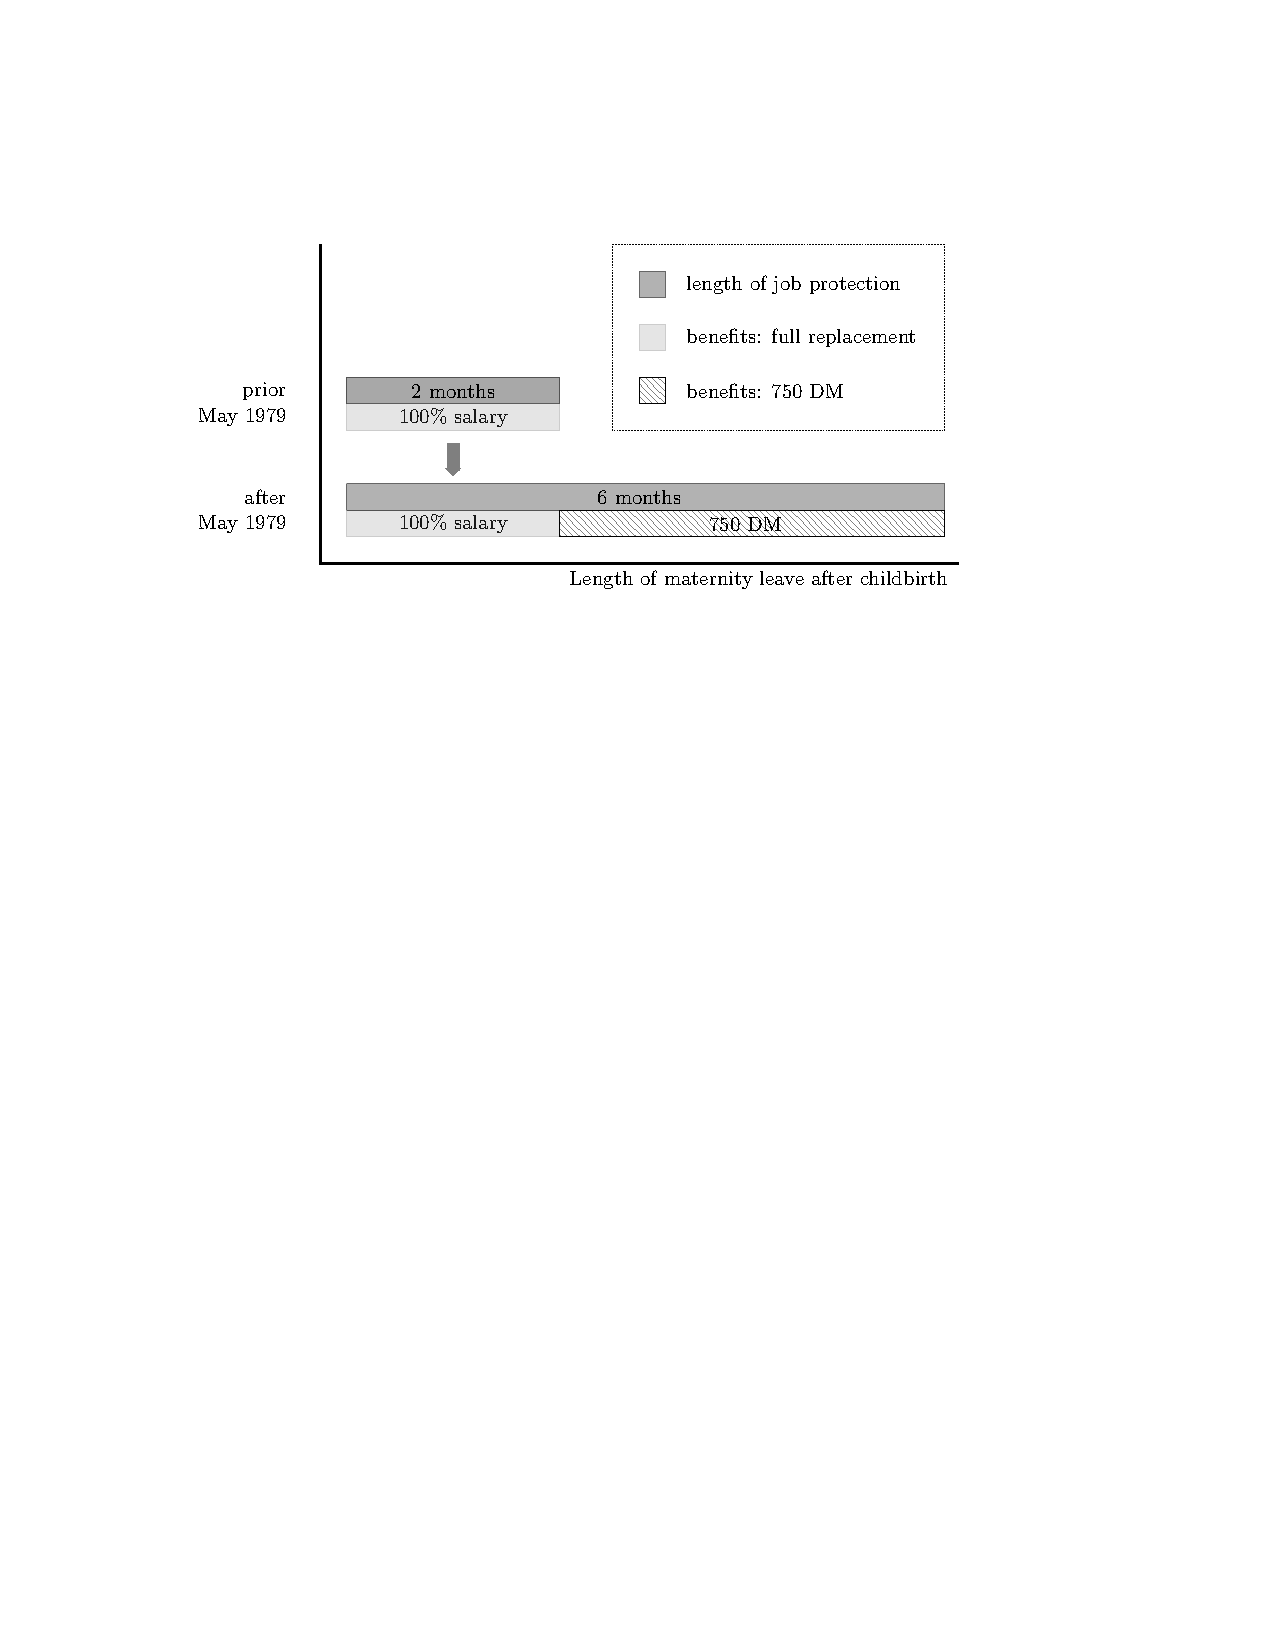
\includegraphics[width=0.8\linewidth]{SOEP/Reform_shortened.pdf}
	\begin{minipage}{\linewidth}
		\scriptsize{\emph{Notes:} The figure describes the legislative change in the length of job protection and maternity leave, which took place in the Federal Republic of Germany in 1979. The reform increased post-birth maternity leave from eight weeks to six months, while keeping the initial structure of the period from six weeks before until eight weeks after childbirth unchanged (mother protection period).\newline \textit{Source: }The figure is based on information from \cite{Dustmann2012}, \cite{DIW2002}, \cite{schonberg2014expansions} as well as \cite{zmarzlik1999mutterschutzgesetz}.}
	\end{minipage}
\end{figure}
%--------------------------------------------
% figure: Bundesgesetzblatt und Familienministerin
\begin{figure}[H]\centering
	\caption{Introduction of the maternity leave law}\label{fig: bundesgesetzblatt_antjehuber}
	\begin{subfigure}[h]{0.48\linewidth}\centering%\caption{Federal law gazette}
		\includegraphics[width=\linewidth]{paper/bundesgesetzblatt_coverpage.png}
	\end{subfigure}
	\begin{subfigure}[h]{0.48\linewidth}\centering%\caption{Federal Minister of Family Affairs Antje Huber} 
	\includegraphics[width=\linewidth]{paper/antje_huber.jpg}
	\end{subfigure}
	\begin{minipage}{\linewidth}
		\scriptsize{\emph{Notes:} On the left, the figure shows the maternity leave law as published in the Federal law gazette. On the right, one can see the Federal Minister of Family affairs Antje Huber at the introduction of the maternity leave law, which was published by the Ministry on the occasion of 30 years of the Federal Ministry of Women.\newline \emph{Source:} Bundesanzeiger Verlag and Federal Ministry of Justice and Consumer Protection (\hyperlink{http://www.bgbl.de/xaver/bgbl/start.xav?startbk=Bundesanzeiger_BGBl&jumpTo=bgbl179s0797.pdf}{BMJV}) and Federal Ministry for Family Affairs, Senior Citizens, Women and Youth (\hyperlink{https://twitter.com/bmfsfj/status/745513281989677058}{BMFSFJ}).}
	\end{minipage}
\end{figure}

%--------------------------------------------


%WMWMWMWMWMWMWMWMWMWMWMWMWMWMWMWMWMWMWMWM
% VALIDITY
%WMWMWMWMWMWMWMWMWMWMWMWMWMWMWMWMWMWMWMWM
\begin{landscape}
	\vspace*{\fill}
	\begin{figure}
		[H]\centering
		\caption{Fertility distribution for different years}\label{fig: fertility_hist}
		\begin{subfigure}[h]{0.40\linewidth}\centering
		\caption{Control: Nov 1977-Oct 1978}
		\includegraphics[width=\linewidth]{paper/fertility_per_day_histogram_CG.pdf}
		\end{subfigure}
		\begin{subfigure}[h]{0.40\linewidth}\centering
		\caption{Treatment: Nov 1978-Oct 1979}
		\includegraphics[width=\linewidth]{paper/fertility_per_day_histogram_TG.pdf}
		\end{subfigure}
			\scriptsize
			\begin{minipage}{0.95\linewidth}
				\emph{Notes:} The figure shows the number of births per day across birth-months for the former region of the Federal Republic of Germany. The solid vertical red line divides pre- and post-reform time span for the treatment group, i.e. two or six months of job-protected leave after childbirth. The dashed line illustrates the same cutoff value for the control group born in other years.\newline
				\emph{Source:} German Federal Statistical Office (Destatis).
			\end{minipage}
	\end{figure}
	\vspace*{\fill}\clearpage
\end{landscape}
%--------------------------------------------
% Fertility distribuition
	\vspace*{\fill}
\begin{figure}[H]\centering
	\caption{Fertility distribution}\label{fig: fertilitydistr}
	\includegraphics[width=0.9\linewidth]{paper/fertility_raw_regression_adjusted.pdf}
	\scriptsize
	\begin{minipage}{0.9 \linewidth}
		\emph{Notes:} 
		 Motivated by \cite{gans2009born} $\rightarrow$ \textbf{how do I get the gray shading from the original figure in the bottom part?}
	\end{minipage}
\end{figure}
\vspace*{\fill}\clearpage

%WMWMWMWMWMWMWMWMWMWMWMWMWMWMWMWMWMWMWMWM
% DATA
%WMWMWMWMWMWMWMWMWMWMWMWMWMWMWMWMWMWMWMWM

% figure: matrix descriptive hospital admission
\newpage
\vspace*{\fill}
\begin{figure}[H]\centering
	\caption{Hospital admissions}\label{fig: descriptive_hospital_admission}
	\includegraphics[width=\linewidth]{paper/descriptive_admission.pdf}
		\begin{minipage}{\linewidth}
		\scriptsize{\emph{Notes:} The figure depicts the evolution of key variables for the treatment cohort (i.e. for individuals born between November 1978 and October 1979) over the period from 1995 to 2014. Hospital admissions are defined as the sum of all diagnoses, except for diagnoses of the "O" chapter (pregnancy, childbirth, and the puerperium). The x-axis shows in addition to the year the age of the treatment cohort in brackets.} 
	\end{minipage}
\end{figure}
\vspace*{\fill}\clearpage
%--------------------------------------------
%figure TOP 5 Diagnoses across age groups
\vspace*{\fill}
\begin{figure}[H]\centering
	\caption{Five main diagnoses of inpatients aged 0 to 35 in 2014}\label{fig: top5diagnosis_in_2014_across_agegroups}
	\includegraphics[width=0.8\linewidth]{paper/top5diagnoses_across_agegroups.pdf}
	\begin{minipage}{\linewidth}
	\scriptsize{\emph{Notes:} The figure shows the incidence distribution across different age brackets of the top five diagnoses for inpatients aged 0 to 35 in 2014. Diagnoses associated with pregnancy, childbirth, and the puerperium are not taken into account in this representation. The large remainder in the age bracket '0-5' consists mostly of conditions that originate in the perinatal period.}
	\end{minipage}
\end{figure}
\vspace*{\fill}\clearpage
%--------------------------------------------



%WMWMWMWMWMWMWMWMWMWMWMWMWMWMWMWMWMWMWMWM
% RESULTS
%WMWMWMWMWMWMWMWMWMWMWMWMWMWMWMWMWMWMWMWM
%--------------------------------------------
\newpage
%Life-course Hospital admission
\begin{landscape}
	\vspace*{\fill}
	\begin{figure}[H]\centering
		\caption{Life-course approach for \textbf{hospital admission}}\label{fig: lc_hospital2_frg_DD}
		\begin{subfigure}[h]{0.31\linewidth}\centering\caption{Total}
			\includegraphics[width=\linewidth]{paper/lc_hospital2_total_gdr.pdf}
		\end{subfigure}
		\begin{subfigure}[h]{0.31\linewidth}\centering\caption{Women}
			\includegraphics[width=\linewidth]{paper/lc_hospital2_female_gdr.pdf}
		\end{subfigure}
		\begin{subfigure}[h]{0.31\linewidth}\centering\caption{Men}
			\includegraphics[width=\linewidth]{paper/lc_hospital2_male_gdr.pdf}
		\end{subfigure}
		\scriptsize
		\begin{minipage}{\linewidth}
			\emph{Notes:} The figures plot DD estimates (along with 90\% and 95\% confidence intervals) for the impact of the reform on hospital admission over the life-course. The light gray line in the background represents the baseline mean of the pre-reform treated cohort. The outcomes are defined as the number of cases per 1,000 individuals (births). Panel a shows the results for all admissions, whereas panel b and c show the estimates for females and males respectively. The control group is comprised of children	that are born in the same months but one year before (i.e. children born between November 1977 and October 1978).
		\end{minipage}
	\end{figure}
	\vspace*{\fill}\clearpage
\end{landscape}
%--------------------------------------------
% HOPSITAL2 - RD plots
%
% Hospital - Reduced form pooled
\newgeometry{left=1cm,right=1cm,top=3cm,bottom=3cm} 
\begin{landscape}
	\vspace*{\fill}
	\begin{figure}
		[H]\centering
		\caption{RD plots for hospital admission (pooled)}\label{fig: rf_hospital2_pooled}
		\begin{subfigure}[h]{0.31\linewidth}\centering\caption{Total}
			\includegraphics[width=\linewidth]{paper/rd_hospital2_total_pooled.pdf}
		\end{subfigure}
		\begin{subfigure}[h]{0.31\linewidth}\centering\caption{Women}
			\includegraphics[width=\linewidth]{paper/rd_hospital2_female_pooled.pdf}
		\end{subfigure}
		\begin{subfigure}[h]{0.31\linewidth}\centering\caption{Men}
			\includegraphics[width=\linewidth]{paper/rd_hospital2_male_pooled.pdf}
		\end{subfigure}
		\scriptsize
		\begin{minipage}{0.95\linewidth}
			\emph{Notes:} The figure plots the average number of diagnoses per 1,000 individuals for month-of-birth cohorts born half a year around the cut-off date of the 1979 maternity leave expansion. The monthly averages are taken over the entire sample length from 1995 to 2014. The dashed lines represent linear fitted values along with 90\%/95\% confidence intervals. The solid vertical red line divides pre- and post-reform schemes (two vs. six months of leave).\newline
			\emph{Source:} Hospital registry data for individuals born between November 1978 and October 1979.
		\end{minipage}
	\end{figure}
	\vspace*{\fill}\clearpage
\end{landscape}
\restoregeometry  
%--------------------------------------------
% Hospital -Reduced form AGE groups 
% original 3 3 2 3
\newgeometry{left=1cm,right=1cm,top=3cm,bottom=3cm} 
\begin{landscape}
	\vspace*{\fill}
	\begin{figure}
		[H]\centering
		\caption{RD plots for hospital admission across age groups}\label{fig: rf_hospital2_agegroup}
		\includegraphics[width=0.85\linewidth]{paper/rd_r_fert_hospital2_overview_agegroups_CIfits.pdf}
		\scriptsize
		\begin{minipage}{0.9\linewidth}
			\emph{Notes:} The figure plots the number of diagnoses per 1,000 individuals for month-of-birth cohorts born half a year around the cut-off date of the 1979 maternity leave expansion across gender and different age groups. The first column reports the ratios for all patients, and the second and third column do so for women and men, respectively. The rows show the ratios across different age groups. The dashed lines represent linear fitted values along with 90\%/95\% confidence intervals. The solid vertical red line divides pre- and post-reform schemes (two vs. six months of leave).\newline
			\emph{Source:} Hospital registry data for individuals born between November 1978 and October 1979.
		\end{minipage}
	\end{figure}
	\vspace*{\fill}\clearpage
\end{landscape}
\restoregeometry

%--------------------------------------------
% Figure: effect sizes and frequency across chapters

\begin{landscape}
	\vspace*{\fill}
	\begin{figure}[H]\centering
		\caption{Intention-to-treat effects across \textbf{main diagnosis chapters}}\label{fig: DD_across_main chapters}
		\begin{subfigure}[h]{0.31\linewidth}\centering\caption{Total}
			\includegraphics[width=\linewidth]{paper/effect_chapters_frequency.pdf}
		\end{subfigure}
		\begin{subfigure}[h]{0.31\linewidth}\centering\caption{Women}
			\includegraphics[width=\linewidth]{paper/effect_chapters_frequency_f.pdf}
		\end{subfigure}
		\begin{subfigure}[h]{0.31\linewidth}\centering\caption{Men}
			\includegraphics[width=\linewidth]{paper/effect_chapters_frequency_m.pdf}
		\end{subfigure}
		\scriptsize
		\begin{minipage}{\linewidth}
			\emph{Notes:} The figures plots intention-to-treat estimates (along with 90\%/95\% confidence intervals) across the main diagnosis chapters. Furthermore, they indicate how often each chapter is diagnosed over the entire time frame (1995-2014). The outcomes are defined as the number of cases per 1,000 individuals (births). The point estimates are coming from a DiD regression as described in section \ref{sec:empirical_strategy}, with a bandwidth of six months, month-of-birth and year fixed effects, and clustered standard errors on the month-of-birth level. The control group is comprised of children	that are born in the same months but one year before the reform (i.e. children born between November 1977 and October 1978). \newline
			\emph{Legend:} Infectious and parasitic diseases (IPD), neoplasms (Neo), mental \& behavioral disorders (MBD), diseases of the nervous system (Ner), diseases of the sense organs (Sen), diseases of the circulatory system (Cir), diseases of the respiratory system (Res), diseases of the digestive system (Dig), diseases of the skin and subcutaneous tissue (SST), diseases of the musculoskeletal system (Mus), diseases of the genitourinary system (Gen), "symptoms, signs, and ill-defined conditions" (Sym), "injury, poisoning and certain other consequences of external causes" (Ext).
			
		\end{minipage}
	\end{figure}
	\vspace*{\fill}\clearpage
\end{landscape}
%--------------------------------------------

% D5 - LC Approach (Mental and behavioral disod)
\begin{landscape}
	\vspace*{\fill}
	\begin{figure}[H]\centering
		\caption{Life-course approach for \textbf{mental and behavioral disorders}}\label{fig: lc_d5_frg_DD}r	\begin{subfigure}[h]{0.31\linewidth}\centering\caption{Total}
			\includegraphics[width=\linewidth]{paper/lc_d5_total_gdr.pdf}
		\end{subfigure}
		\begin{subfigure}[h]{0.31\linewidth}\centering\caption{Women}
			\includegraphics[width=\linewidth]{paper/lc_d5_female_gdr.pdf}
		\end{subfigure}
		\quad
		\begin{subfigure}[h]{0.31\linewidth}\centering\caption{Men}
			\includegraphics[width=\linewidth]{paper/lc_d5_male_gdr.pdf}
		\end{subfigure}
		\scriptsize
		\begin{minipage}{\linewidth}
			\emph{Notes:} The figures plot DD estimates (along with 90\% and 95\% confidence intervals) for the impact of the reform on mental and behavioral disorders over the life-course. The light gray line in the background represents the baseline mean of the pre-reform treated cohort. The outcomes are defined as the number of cases per 1,000 individuals (births). Panel a shows the results for all admissions, whereas panel b and c show the estimates for females and males respectively. The control group is comprised of children	that are born in the same months but one year before (i.e. children born between November 1977 and October 1978).
		\end{minipage}
	\end{figure}
	\vspace*{\fill}\clearpage
\end{landscape}

%--------------------------------------------
% D5 RD plots
%
% d5 - RF pooled
\newgeometry{left=1cm,right=1cm,top=3cm,bottom=3cm} 
\begin{landscape}
	\vspace*{\fill}
	\begin{figure}
		[H]\centering
		\caption{RD plots for mental \& behavioral disorders (pooled)}\label{fig: rf_d5_pooled}
		\begin{subfigure}[h]{0.31\linewidth}\centering\caption{Total}
			\includegraphics[width=\linewidth]{paper/rd_d5_total_pooled.pdf}
		\end{subfigure}
		\begin{subfigure}[h]{0.31\linewidth}\centering\caption{Women}
			\includegraphics[width=\linewidth]{paper/rd_d5_female_pooled.pdf}
		\end{subfigure}
		\begin{subfigure}[h]{0.31\linewidth}\centering\caption{Men}
			\includegraphics[width=\linewidth]{paper/rd_d5_male_pooled.pdf}
		\end{subfigure}
		\scriptsize
		\begin{minipage}{0.95\linewidth}
			\emph{Notes:} The figure plots the average number of diagnoses per 1,000 individuals for month-of-birth cohorts born half a year around the cut-off date of the 1979 maternity leave expansion. The monthly averages are taken over the entire sample length from 1995 to 2014. The dashed lines represent linear fitted values along with 90\%/95\% confidence intervals. The solid vertical red line divides pre- and post-reform schemes (two vs. six months of leave).\newline
			\emph{Source:} Hospital registry data for individuals born between November 1978 and October 1979.
		\end{minipage}
	\end{figure}
	\vspace*{\fill}\clearpage
\end{landscape}
\restoregeometry 




%--------------------------------------------
% D5 - RF (age group)
\newgeometry{left=1cm,right=1cm,top=3cm,bottom=3cm} 
\begin{landscape}
	\vspace*{\fill}
	\begin{figure}
		[H]\centering
		\caption{RD plots for mental \& behavioral disorders across age groups}\label{fig: rf_d5_agegroup}
		\includegraphics[width=0.85\linewidth]{paper/rd_r_fert_d5_overview_agegroups_CIfits.pdf}
		\scriptsize
		\begin{minipage}{0.9\linewidth}
			\emph{Notes:} The figure plots the number of diagnoses per 1,000 individuals for month-of-birth cohorts born half a year around the cut-off date of the 1979 maternity leave expansion across gender and different age groups. The first column reports the ratios for all patients, and the second and third column do so for women and men, respectively. The rows show the ratios across different age groups. The dashed lines represent linear fitted values along with 90\%/95\% confidence intervals. The solid vertical red line divides pre- and post-reform schemes (two vs. six months of leave).\newline
			\emph{Source:} Hospital registry data for individuals born between November 1978 and October 1979.
		\end{minipage}
	\end{figure}
	\vspace*{\fill}\clearpage
\end{landscape}
\restoregeometry

  
%--------------------------------------------
% Graph D5 partition - Subcategories
\vspace*{\fill}
\begin{figure}[H]\centering
	\caption{The top five subcategories of mental \& behavioral diagnoses}\label{fig: d5partition}
	\includegraphics[width=0.8\linewidth]{../../analysis/graphs/paper/d5partition_lfstat.pdf}
	\scriptsize
	\begin{minipage}{0.9\linewidth}
	\emph{Notes:} This figure plots the yearly number of diagnoses for the treatment cohort (i.e. the individuals born between November 1978 and October 1979). The subcategories are ordered by their occurrence in 2014 (from the most to the least frequent diagnosis), which also coincides by chance with the ordering in the ICD-10 classification system. The five most frequent subcategories - as shown here - comprise more than 95\% of all mental and behavioral disorders. 
	\end{minipage}
\end{figure}
\vspace*{\fill}\clearpage%--------------------------------------------
% figure: iverview of d5 subcategories (effects + frequency)
\newgeometry{left=1cm,right=1cm,top=3cm,bottom=3cm} 
\begin{landscape}
	\vspace*{\fill}
	\begin{figure}
		[H]\centering
		\caption{ITT effect for \textbf{subcategories of mental \& behavioral disorders (pooled)}}\label{fig: ITT_d5_subcategories}
		\begin{subfigure}[h]{0.31\linewidth}\centering\caption{Total}
			\includegraphics[width=\linewidth]{paper/effect_d5_frequency.pdf}
		\end{subfigure}
		\begin{subfigure}[h]{0.31\linewidth}\centering\caption{Women}
			\includegraphics[width=\linewidth]{paper/effect_d5_frequency_f.pdf}
		\end{subfigure}
		\begin{subfigure}[h]{0.31\linewidth}\centering\caption{Men}
			\includegraphics[width=\linewidth]{paper/effect_d5_frequency_m.pdf}
		\end{subfigure}
		\scriptsize
		\begin{minipage}{0.95\linewidth}
			\emph{Notes:} The figure plots ITT estimates (along with 90\%/95\% confidence intervals) across the five most common subcategories of mental and behavioral disorders. Moreover, they indicate how often each subcategory is diagnosed over the time window of 1995-2014. The outcomes are defined as the number of cases per 1,000 individuals (births). The point estimates are coming from a DiD regression as described in section \ref{sec:empirical_strategy}, with a bandwidth of six months, month-of-birth and year fixed effects, and standard errors clustered at the month-of-birth level. The control group is comprised of children that are born in the same months but one year before the reform (i.e. children born between November 1977 and October 1978).\newline
			\emph{Source:} Hospital registry data.
		\end{minipage}
	\end{figure}
	\vspace*{\fill}\clearpage
\end{landscape}
\restoregeometry 






%--------------------------------------------------------------------
% TABLES
%--------------------------------------------------------------------
\newpage
\TODO\section{Tables}
\vspace*{\fill}
{\Huge \begin{center}\textbf{TABLES}\end{center}}
\vspace*{\fill}\clearpage

%--------------------------------------------
% Overview ICD 9 and ICD 10 
%\begin{small}
%\vspace*{\fill}
%\begin{table}[h] % table environment for caption and label
%	\begin{threeparttable}
%		\centering % center the tabular
%		\caption{Overview of diagnoses} % caption
%		\label{tab:outcomes_coding_main_chapters} 
%		\begin{tabular}{lrrr} % alignment and number of columns of actual table
%			\toprule % top thicker horizontal line (" rule ")
%			&\multicolumn{1}{r}{(1)}& &\multicolumn{1}{r}{(2)}\\
%			&\multicolumn{1}{r}{ICD-9} & & \multicolumn{1}{r}{ICD-10} \\ 
%			\midrule
%			%-------------------------------------------------------------------------
%			\textit{Main diagnosis chapters}\\
 \hspace{4pt} Infectious and parasitic diseases                           	&	001-139		& &		A00-B99 \\
 \hspace{4pt} Neoplasms                                                   	&	140-239		& &		C00-D48 \\
%\hspace{4pt} Diseases of the blood and blood-forming organs              	&	280-289		& &		D50-D90 \\
 \hspace{4pt} Endocrine, nutritional and metabolic diseases					&	240-278		& &		E00-E90 \\
 \hspace{4pt} Mental \& behavioral  disorders                             	&	290-319		& &		F00-F99 \\
 \hspace{4pt} Diseases of the nervous system                              	&	320-359		& &		G00-G99 \\
 \hspace{4pt} Diseases of the sense organs                                	&	360-389		& &		H00-H95 \\
 \hspace{4pt} Diseases of the circulatory system                          	&	390-459		& &		I00-I99 \\
 \hspace{4pt} Diseases of the respiratory system                          	&	460-519		& &		J00-J99 \\
 \hspace{4pt} Diseases of the digestive system                            	&	520-579		& &		K00-K93 \\
 \hspace{4pt} Diseases of the skin and subcutaneous tissue                	&	680-709		& &		L00-L99 \\
 \hspace{4pt} Diseases of the musculoskeletal system and connective tissue	&	710-739		& &		M00-M99 \\
 \hspace{4pt} Diseases of the genitourinary system                        	&	580-629		& &		N00-N99 \\
 \hspace{4pt} Complications of pregnancy, childbirth, and the puerperium  	&	630-676		& &		O00-O99 \\
%\hspace{4pt} Certain conditions originating in the perinatal period      	&	760-779		& &		P00-P96 \\
%\hspace{4pt} Congenital anomalies                                        	&	740-759		& &		Q00-Q99 \\
 \hspace{4pt} Symptoms, signs, and ill-defined conditions                 	&	780-799		& &		R00-R99 \\
 \hspace{4pt} Injury and poisoning                                        	&	800-999		& &		S00-T98 \\
 \\
 \textit{}

\
%			%-------------------------------------------------------------------------
%			\bottomrule % bottom thicker horizontal line (" rule ")
%		\end{tabular}
%		\begin{tablenotes}
%			\scriptsize{ \item \textit{Notes:} The table shows the classification of diseases according to the "International Statistical Classification of Diseases and Related Health Problems (ICD)", a medical classification list provided by the World Health Organization. \newline \textit{Source:} World Health Organization (WHO), see for example: \href{http://www.who.int/classifications/icd/en/}{http://www.who.int/classifications/icd/en/}\newline$^1$ Psychoactive substances include alcohol, opioids, cannabinoids, sedatives or hypnotics, cocaine, other stimulants (including caffeine), hallucinogens, tobacco, volatile solvents,  multiple drug use and use of other psychoactive substances. }
%		\end{tablenotes}
%	\end{threeparttable}
%\end{table}
%\vspace*{\fill}\clearpage 
%%\end{small}
%%\normalsize


%--------------------------------------------
% Overview Hopsital admission
\newgeometry{left=0cm,right=0cm,top=0cm,bottom=3cm} 

\begin{landscape}
	\vspace*{\fill}
	\begin{table}[h] \centering % table environment for caption and label
		\begin{threeparttable}
			\centering % center the tabular
			\caption{Summary statistics for different diagnoses} % caption
			\label{tab:outcomes_coding_main_chapters} 
			\begin{tabular}{lrrrrrr} % alignment and number of columns of actual table
				\toprule % top thicker horizontal line (" rule ")
				&\multicolumn{1}{r}{(1)}& &\multicolumn{1}{r}{(2)}&\multicolumn{1}{r}{(3)} &\multicolumn{1}{r}{(4)}\\
				&\multicolumn{1}{r}{ICD-9} & & \multicolumn{1}{r}{ICD-10}&\multicolumn{1}{r}{Mean}&\multicolumn{1}{r}{SD} \\ 
				\midrule
				%-------------------------------------------------------------------------
				\\
\underline{\textit{A. Hospital admission}}									& 						& & 			 & 	 120.625     &  10.961\\ 
 \hspace{10pt} Infectious and parasitic diseases                           	&	001-139				& &		A00-B99  & 	   4.210     &   0.493\\
 \hspace{10pt} Neoplasms                                                   	&	140-239				& &		C00-D48  & 	   5.155     &   1.282\\
 \hspace{10pt} Mental \& behavioral  disorders                             	&	290-319				& &		F00-F99  & 	  18.956     &   5.548\\
 \hspace{10pt} Diseases of the nervous system                              	&	320-359				& &		G00-G99  & 	   4.500     &   1.264\\
 \hspace{10pt} Diseases of the sense organs                                	&	360-389				& &		H00-H95  & 	   2.404     &   0.348\\
 \hspace{10pt} Diseases of the circulatory system                          	&	390-459				& &		I00-I99  & 	   4.108     &   1.380\\
 \hspace{10pt} Diseases of the respiratory system                          	&	460-519				& &		J00-J99  & 	  10.994     &   1.939\\
 \hspace{10pt} Diseases of the digestive system                            	&	520-579				& &		K00-K93  & 	  16.746     &   2.079\\
 \hspace{10pt} Diseases of the skin and subcutaneous tissue                	&	680-709				& &		L00-L99  & 	   3.849     &   0.536\\
 \hspace{10pt} Diseases of the musculoskeletal system						&	710-739				& &		M00-M99  & 	   8.897     &   2.228\\
 \hspace{10pt} Diseases of the genitourinary system                        	&	580-629				& &		N00-N99  & 	  10.621     &   1.362\\
 \hspace{10pt} Symptoms, signs, and ill-defined conditions                 	&	780-799				& &		R00-R99  & 	   6.794     &   1.410\\
 \hspace{10pt} Injury, poisoning and certain other                          &	800-999				& &		S00-T98  & 	  21.196     &   5.978\\
 \hspace{18pt} consequences of external causes  \\
 
 %\hspace{4pt} Diseases of the blood and blood-forming organs              	&	280-289		& &		D50-D90  & \\
 %\hspace{4pt} Endocrine, nutritional and metabolic diseases				&	240-278		& &		E00-E90  & \\
 %\hspace{4pt} Pregnancy, childbirth, and the puerperium  					&	630-676		& &		O00-O99  & \\
 %\hspace{4pt} Certain conditions originating in the perinatal period      	&	760-779		& &		P00-P96  & \\
 %\hspace{4pt} Congenital anomalies                                        	&	740-759		& &		Q00-Q99  & \\
 
 
 % ------------------------------------------------------------------------
 % 							Mean           SD          Min          Max
 % ------------------------------------------------------------------------
 % Ratio using number~e      120.625       10.961        99.27       156.35
 % Ratio using number~e        4.210        0.493         2.87         5.65
 % Ratio using number~e        5.155        1.282         3.29         8.97
 % Ratio using number~e       18.956        5.548         6.68        30.17
 % Ratio using number~e        4.500        1.264         2.60         7.50
 % Ratio using number~e        2.404        0.348         1.62         3.07
 % Ratio using number~e        4.108        1.380         1.41         7.66
 % Ratio using number~e       10.994        1.939         8.30        15.55
 % Ratio using number~e       16.746        2.079        12.09        20.97
 % Ratio using number~e        3.849        0.536         2.63         5.12
 % Ratio using number~e        8.897        2.228         6.45        15.46
 % Ratio using number~e       10.621        1.362         6.79        13.64
 % Ratio using number~e        6.794        1.410         4.26        10.70
 % Ratio using number~e       21.196        5.978        14.41        34.06
 % ------------------------------------------------------------------------



				%-------------------------------------------------------------------------
				\bottomrule % bottom thicker horizontal line (" rule ")
			\end{tabular}
			\begin{tablenotes}
				\scriptsize{ \item \textit{Continued on next page}}
			\end{tablenotes}
		\end{threeparttable}
	\end{table}
	\vspace*{\fill}\clearpage 
	
	
	\vspace*{\fill}
	\begin{table}[h] \centering % table environment for caption and label
		\begin{threeparttable}
			\centering % center the tabular
			\caption*{\textit{Summary statistics for different diagnoses (continued)}} % caption

			\begin{tabular}{lrrrrrr} % alignment and number of columns of actual table
				\toprule % top thicker horizontal line (" rule ")
				&\multicolumn{1}{r}{(1)}& &\multicolumn{1}{r}{(2)}&\multicolumn{1}{r}{(3)} &\multicolumn{1}{r}{(4)}\\
				&\multicolumn{1}{r}{ICD-9} & & \multicolumn{1}{r}{ICD-10}&\multicolumn{1}{r}{Mean}&\multicolumn{1}{r}{SD} \\ 
				\midrule
				%-------------------------------------------------------------------------
				

\\
\underline{\textit{B. Mental \& behavioral disorders}}						&						& & 			 & 18.956		& 5.548		\\
 \hspace{10pt} Organic, including symptomatic, mental disorders				& 290,293,294,310		& & 	F00-F09	 &	0.115		& 0.056		\\
 \hspace{10pt} MBD due to psychoactive substance use$^1$					& 291,292,303,304,305	& & 	F10-F19	 &	6.366		& 2.232		\\
 \hspace{10pt} Schizophrenia, schizotypal and delusional disorders			& 295,297,298			& & 	F20-F29	 &	5.140		& 2.246		\\
 \hspace{10pt} Mood [affective] disorders									& 296,311				& & 	F30-F39	 &	2.339		& 1.673		\\
 \hspace{10pt} Neurotic, stress-related and somatoform disorders			& 300,306,308,309		& & 	F40-F48	 &	2.799		& 0.356		\\
 \hspace{10pt} Behavioural syndromes associated with 						& 316					& & 	F50-F59	 &	0.308		& 0.225		\\
 \hspace{18pt} physiological disturbances and physical factors 														 &				& 			\\
 \hspace{10pt} Disorders of adult personality and behavior					& 301,302				& & 	F60-F69	 &	1.375		& 0.511		\\
 \hspace{10pt} Mental retardation 											& 317,318,319			& &		F70-F79	 &	0.121		& 0.075		\\
 \hspace{10pt} Disorders of psychological development						& 299,315				& & 	F80-F89	 &	0.026		& 0.029		\\
 \hspace{10pt} Behavioural and emotional disorders with 					& 312,313,314,307		& & 	F90-F98	 &	0.320		& 0.535		\\
  \hspace{18pt} onset usually occurring in childhood and adolescence 																			\\


% var			mean	SD
% d5						18.956	5.548
% organic					0.115	0.056
% psychoactive substances	6.366	2.232
% schizophrenia			5.140	2.246
% affective				2.339	1.673
% neurosis				2.799	0.356
% physical factors		0.308	0.225
% personality				1.375	0.511
% retardation				0.121	0.075
% development				0.026	0.029
% childhood				0.320	0.535
		


				%-------------------------------------------------------------------------
				\bottomrule % bottom thicker horizontal line (" rule ")
			\end{tabular}
			\begin{tablenotes}
				\scriptsize{ \item \textit{Notes:} The table shows the classification of diseases according to the "International Statistical Classification of Diseases and Related Health Problems (ICD)", a medical classification list provided by the World Health Organization.  The table reports next to the ICD codes summary statistics for the different diagnosis types. Column 3 and 4 show mean and standard deviation of the number of diagnosis per 1,000 individuals for the pre-reform treatment cohort. \newline \textit{Source:} World Health Organization (WHO), see for example: \href{http://www.who.int/classifications/icd/en/}{http://www.who.int/classifications/icd/en/} for the ICD coding, hospital registry data for the mean and standard deviation. \newline\hspace*{15 pt}$^1$ Psychoactive substances include alcohol, opioids, cannabinoids, sedatives or hypnotics, cocaine, other stimulants (including caffeine), hallucinogens, tobacco, volatile solvents,  multiple drug use and use of other psychoactive substances. }
			\end{tablenotes}
		\end{threeparttable}
	\end{table}
	\vspace*{\fill}\clearpage 
\end{landscape}
\restoregeometry
%--------------------------------------------
%VALIDITY: Birth rate effects
 \vspace*{\fill}
 \begin{table}[H] \centering
 \caption{Validity: birth rate effects}\label{tab: validity_birth_rate}
 {\def\sym#1{\ifmmode^{#1}\else\(^{#1}\)\fi} 
 \begin{tabular}{l*{5}{c}}
 	\toprule
 	& \multicolumn{4}{c}{Estimation window} \\
 	\cmidrule{2-5}
 	&\multicolumn{1}{c}{(1)}&\multicolumn{1}{c}{(2)}&\multicolumn{1}{c}{(3)}&\multicolumn{1}{c}{(4)}\\
	 & \multicolumn{1}{c}{$\pm$7 days} & \multicolumn{1}{c}{$\pm$14 days} & \multicolumn{1}{c}{$\pm$21 days} & \multicolumn{1}{c}{$\pm$28 days}\\ 
 	\midrule
 	\multicolumn{5}{l}{\emph{Panel A. Dependent variable is number of births}}\\
 	ML reform           &      -30.46         &      -30.23\sym{*}  &      -33.32\sym{**} &      -32.78\sym{***}\\
                    &     (30.31)         &     (17.73)         &     (14.08)         &     (12.37)         \\
Observations        &         196         &         392         &         588         &         784         \\
$R^2$               &       0.856         &       0.842         &       0.832         &       0.817         \\

 	\\ \\
 	\multicolumn{5}{l}{\emph{Panel B. Dependent variable is ln(number of births)}}\\
 	ML reform           &     -0.0448         &     -0.0440\sym{*}  &     -0.0477\sym{**} &     -0.0476\sym{***}\\
                    &    (0.0425)         &    (0.0247)         &    (0.0197)         &    (0.0173)         \\
Observations        &         196         &         392         &         588         &         784         \\
$R^2$               &       0.855         &       0.844         &       0.833         &       0.819         \\

 	\bottomrule
 \end{tabular}}
 \begin{minipage}{0.9\linewidth}
 		\scriptsize \emph{Notes:} 
 	\end{minipage}
 \end{table}
 \vspace*{\fill}\clearpage 

%--------------------------------------------
% HOSPITAL - Difference in Difference tables for 
\newpage

\begin{table}[t] \centering 
 \begin{threeparttable} \centering \caption{ITT effects on hospital admission}\label{tab_mlch: DD_hopsital2_total}
  {\def\sym#1{\ifmmode^{#1}\else\(^{#1}\)\fi} 
 	\begin{tabular}{l*{6}{c}}
 		\toprule 
 		%\multicolumn{5}{l}{Dependant variable: \textbf{Hospital admission (total)}}\\ \\ 
 		& \multicolumn{5}{c}{Estimation window} \\ 
 		\cmidrule(lr){2-6}
 		&\multicolumn{1}{c}{(1)}&\multicolumn{1}{c}{(2)}&\multicolumn{1}{c}{(3)}&\multicolumn{1}{c}{(4)}&\multicolumn{1}{c}{(5)}\\
 		&\multicolumn{1}{c}{6M}&\multicolumn{1}{c}{5M}&\multicolumn{1}{c}{4M}&\multicolumn{1}{c}{3M}&\multicolumn{1}{c}{Donut}\\
 		\midrule
 		\multicolumn{5}{l}{\emph{Panel A. Over entire length of the life-course}} \\
 		\hspace*{10pt}Overall&      -2.218         &      -2.181\sym{*}  &      -1.944\sym{**} &      -2.168\sym{**} &      -2.713\sym{***}\\
                    &     (1.401)         &     (1.143)         &     (0.917)         &     (0.782)         &     (0.826)         \\
\midrule Dependent mean&       122.7         &       121.0         &       120.5         &       120.6         &       121.4         \\
Effect in SDs [\%]  &       19.22         &       18.84         &       17.35         &       19.78         &       24.62         \\
Observations        &         240         &         320         &         400         &         480         &         400         \\
 \\ \\
 		\multicolumn{5}{l}{\emph{Panel B. Age brackets}} \\
 		\hspace*{10pt}Age 17-21&      -1.095         &      -0.735         &      -0.590         &      -1.517\sym{+}  &      -1.963\sym{**} \\
                    &     (1.603)         &     (1.198)         &     (0.995)         &     (0.946)         &     (0.931)         \\
 \hspace*{10pt}Age 22-26&      -0.735         &      -0.667         &      -0.613         &      -0.611         &      -1.080         \\
                    &     (1.672)         &     (1.412)         &     (1.113)         &     (0.937)         &     (1.012)         \\
 \hspace*{10pt}Age 27-31&      -2.546\sym{*}  &      -3.209\sym{**} &      -3.015\sym{***}&      -2.665\sym{***}&      -2.974\sym{***}\\
                    &     (1.375)         &     (1.132)         &     (0.909)         &     (0.826)         &     (0.949)         \\
 \hspace*{10pt}Age 32-35&      -3.869\sym{***}&      -3.619\sym{**} &      -4.572\sym{***}&      -5.045\sym{**} &      -4.717\sym{***}\\
                    &     (1.083)         &     (1.277)         &     (1.460)         &     (1.721)         &     (1.191)         \\
 
 		\bottomrule 
 	\end{tabular}}
 	\begin{tablenotes} 
 		\item \scriptsize \emph{Notes:} The table shows DiD estimates of the 1979 maternity leave reform on hospital admission for different estimation windows around the cutoff. The \textit{`Donut'} specification uses a bandwidth of half a year and excludes children born in April and May. Panel A shows the effect for the entire pooled time frame and panel B reports estimates per age bracket. The outcome variables are defined as the number of cases per thousand individuals. All regressions control for year and month-of-birth fixed effects. The control group is comprised of children that are born in the same months but one year before the reform (i.e. children born between November 1977 and October 1978). In order to compare the two birth cohorts at the same age, I shift the control cohort from wave $t$ to wave $t+1$. The dependent mean and the effect size in standard deviation units correspond to pre-reform values of the treated group. Table \ref{tab_mlch: observations_age_brackets} contains the number of observations for the estimations per age bracket. Clustered standard errors are reported in parentheses. \newline Significance levels: * p < 0.10, ** p < 0.05, *** p < 0.01. \newline 	%\emph{Source:} Hospital registry data.
 	\end{tablenotes} 
 \end{threeparttable} 
 \end{table}
\vspace*{\fill}
 \begin{table}[H] \centering 
 	\begin{threeparttable} \centering \caption{ITT effects on \textbf{hospital admission (women)}}\label{tab: DD_hopsital2_female} {\def\sym#1{\ifmmode^{#1}\else\(^{#1}\)\fi} 
 			\begin{tabular}{l*{6}{c}}
 				\toprule 
 				%\multicolumn{5}{l}{Dependant variable: \textbf{Hospital admission (total)}}\\ \\ 
 				& \multicolumn{5}{c}{Estimation window} \\ 
 				\cmidrule(lr){2-6}
 				&\multicolumn{1}{c}{(1)}&\multicolumn{1}{c}{(2)}&\multicolumn{1}{c}{(3)}&\multicolumn{1}{c}{(4)}&\multicolumn{1}{c}{(5)}\\
 				&\multicolumn{1}{c}{6M}&\multicolumn{1}{c}{5M}&\multicolumn{1}{c}{4M}&\multicolumn{1}{c}{3M}&\multicolumn{1}{c}{Donut}\\
 				\midrule
 				\multicolumn{5}{l}{\emph{Panel A.Over entire length of the life-course}} \\
 				\hspace*{10pt}Overall&       0.149         &      -0.766         &      -1.815\sym{**} &      -2.278\sym{***}\\
                    &     (2.038)         &     (1.088)         &     (0.807)         &     (0.751)         \\
\midrule Dependent mean&       122.3         &       122.0         &       122.4         &       123.3         \\
Effect in SDs [\%]  &       1.350         &       6.530         &       16.29         &       20.28         \\
Observations        &         160         &         320         &         480         &         400         \\
 \\ \\
 				\multicolumn{5}{l}{\emph{Panel B. Age brackets}} \\
 				\hspace*{10pt}Age 17-21&      -2.121\sym{+}  &      -1.274         &      -1.931\sym{*}  &      -2.916\sym{***}&      -3.322\sym{***}\\
                    &     (1.269)         &     (1.018)         &     (0.959)         &     (0.935)         &     (0.985)         \\
 \hspace*{10pt}Age 22-26&       1.661         &       1.126         &      0.0274         &      -0.510         \\
                    &     (3.675)         &     (1.806)         &     (1.267)         &     (1.117)         \\
 \hspace*{10pt}Age 27-31&      -1.379         &      -1.669         &      -2.605\sym{**} &      -2.762\sym{**} &      -2.944\sym{***}\\
                    &     (1.765)         &     (1.336)         &     (1.163)         &     (1.004)         &     (0.917)         \\
 \hspace*{10pt}Age 32-35&      -0.605         &      -1.004         &      -0.841         &      -1.212         &      -1.810\sym{*}  \\
                    &     (1.300)         &     (1.165)         &     (1.024)         &     (0.866)         &     (0.941)         \\
 
 				\bottomrule 
 		\end{tabular}}
 		\begin{tablenotes} 
 			\item \scriptsize \emph{Notes:} The table shows DiD estimates of the 1979 maternity leave reform on hospital admission for different estimation windows around the cutoff. The \textit{`Donut'} specification uses a bandwidth of half a year and excludes children born in April and May. Panel A shows the effect for the entire pooled time frame and panel B breaks the life-course up in age brackets. The outcome variables are defined as the number of cases per thousand individuals (births). All regressions control for year and month-of-birth fixed effects. The control group is comprised of children that are born in the same months but one year before the reform (i.e. children born between November 1977 and October 1978). In order to compare the two birth cohorts at the same age, I shift the control cohort from wave $t$ to wave $t+1$. The dependent mean and the effect size in standard deviation units correspond to pre-reform values of the treated group. Clustered standard errors are reported in parentheses. \newline Significance levels: + p < 0.15, * p < 0.10, ** p < 0.05, *** p < 0.01. \newline 	\emph{Source:} Hospital registry data.
 		\end{tablenotes} 
 	\end{threeparttable} 
 \end{table}
\vspace*{\fill}\clearpage 
 \vspace*{\fill}
 \begin{table}[H] \centering 
 	\begin{threeparttable} \centering \caption{ITT effects on \textbf{hospital admission (men)}}\label{tab: DD_hopsital2_male} {\def\sym#1{\ifmmode^{#1}\else\(^{#1}\)\fi} 
 		\begin{tabular}{l*{6}{c}}
 			\toprule 
 			%\multicolumn{5}{l}{Dependant variable: \textbf{Hospital admission (total)}}\\ \\ 
 			& \multicolumn{5}{c}{Estimation window} \\ 
 			\cmidrule(lr){2-6}
 			&\multicolumn{1}{c}{(1)}&\multicolumn{1}{c}{(2)}&\multicolumn{1}{c}{(3)}&\multicolumn{1}{c}{(4)}&\multicolumn{1}{c}{(5)}\\
 			&\multicolumn{1}{c}{6M}&\multicolumn{1}{c}{5M}&\multicolumn{1}{c}{4M}&\multicolumn{1}{c}{3M}&\multicolumn{1}{c}{Donut}\\
 				\midrule
 				\multicolumn{5}{l}{\emph{Panel A. Over entire length of the life-course}} \\
 				\hspace*{10pt}Overall&      -0.445         &      -3.528\sym{**} &      -2.525\sym{**} &      -3.148\sym{**} \\
                    &     (1.017)         &     (1.387)         &     (0.997)         &     (1.144)         \\
\midrule Dependent mean&       118.3         &       120.0         &       118.9         &       119.7         \\
Effect in SDs [\%]  &       3.440         &       25.82         &       19.34         &       23.95         \\
Observations        &         160         &         320         &         480         &         400         \\
 \\ \\
 				\multicolumn{5}{l}{\emph{Panel B. Age brackets}} \\
 				\hspace*{10pt}Age 17-21&      -0.157         &      -0.246         &       0.634         &      -0.273         &      -0.757         \\
                    &     (2.147)         &     (1.592)         &     (1.344)         &     (1.201)         &     (1.241)         \\
 \hspace*{10pt}Age 22-26&       0.918         &      -2.373         &      -1.230         &      -1.633         \\
                    &     (0.719)         &     (1.497)         &     (1.048)         &     (1.241)         \\
 \hspace*{10pt}Age 27-31&      -0.652\sym{***}&      -4.669\sym{**} &      -2.558\sym{*}  &      -2.987\sym{*}  \\
                    &     (0.106)         &     (1.625)         &     (1.294)         &     (1.528)         \\
 \hspace*{10pt}Age 32-35&      -5.852\sym{**} &      -7.955\sym{***}&      -6.373\sym{***}&      -7.461\sym{***}\\
                    &     (2.312)         &     (1.969)         &     (1.526)         &     (1.722)         \\
 
 				\bottomrule 
 		\end{tabular}}
 		\begin{tablenotes} 
 			\item \scriptsize \emph{Notes:} The table shows DD estimates of the 1979 maternity leave reform on hospital admission for different bandwidths around the cutoff. Panel A shows the effect for the entire pooled time frame and panel B breaks the life-course up in age brackets. The outcome variables are defined as the number of cases per thousand individuals (births). All regressions control for year and month-of-birth fixed effects. The control group is comprised of children that are born in the same months but one year before the reform (i.e. children born between November 1977 and October 1978). In order to compare the two birth cohorts at the same age, we shift the control cohort from wave $t$ to wave $t+1$. The dependent mean and the effect size in standard deviation units correspond to pre-reform values of the treated group. Clustered standard errors are reported in parentheses. \newline Significance levels: + p < 0.15, * p < 0.10, ** p < 0.05, *** p < 0.01. \newline 	\emph{Source:} Hospital registry data.
 		\end{tablenotes} 
 	\end{threeparttable} 
 \end{table} 
\vspace*{\fill}\clearpage 

%--------------------------------------------
% ITT effects nach chaptern
% original 3 3 2 3
\newpage
\newgeometry{left=3cm,right=3cm,top=1cm,bottom=2.5cm} 
\vspace*{\fill}
\begin{table}[H] \centering 
	\begin{threeparttable} \centering \caption{ITT effects on \textbf{hospital admission and main diagnoses chapters (total)}}\label{tab: ITT_across_chapters_per_age_group_total}
		{\def\sym#1{\ifmmode^{#1}\else\(^{#1}\)\fi} 
			\begin{tabular}{l*{5}{c}}
				\toprule 
				&\multicolumn{1}{c}{(1)}&\multicolumn{1}{c}{(2)}&\multicolumn{1}{c}{(3)}&\multicolumn{1}{c}{(4)}&\multicolumn{1}{c}{(5)}\\
				\midrule
				&\multirow{2}{*}{Overall} & \multicolumn{4}{c}{Age brackets [years]} \\ 
				\cmidrule(lr){3-6}
				&&\multicolumn{1}{c}{17-21}&\multicolumn{1}{c}{22-26}&\multicolumn{1}{c}{27-31}&\multicolumn{1}{c}{32-35}\\
				
				\midrule
				
				Hospital            &      -2.168\sym{**} &      -1.517         &      -0.611         &      -2.665\sym{***}&      -3.869\sym{***}\\
                    &     (0.782)         &     (0.946)         &     (0.937)         &     (0.826)         &     (1.083)         \\
IPD                 &     -0.0838\sym{**} &      0.0130         &      -0.162         &      -0.126\sym{**} &     -0.0197         \\
                    &    (0.0334)         &    (0.0680)         &     (0.108)         &    (0.0548)         &     (0.111)         \\
Neo                 &      0.0269         &      -0.198         &       0.336\sym{**} &       0.121         &      -0.217         \\
                    &    (0.0821)         &     (0.155)         &     (0.139)         &     (0.102)         &     (0.164)         \\
MBD                 &      -0.634\sym{**} &       0.174         &    -0.00769         &      -1.000\sym{**} &      -1.906\sym{***}\\
                    &     (0.249)         &     (0.263)         &     (0.420)         &     (0.357)         &     (0.372)         \\
Ner                 &     0.00791         &     -0.0919         &       0.238\sym{***}&      0.0374         &     -0.0190         \\
                    &    (0.0561)         &    (0.0558)         &    (0.0751)         &    (0.0963)         &     (0.126)         \\
Sen                 &      -0.144\sym{***}&      -0.168\sym{**} &     -0.0990\sym{*}  &      -0.172\sym{**} &      -0.261\sym{**} \\
                    &    (0.0272)         &    (0.0626)         &    (0.0518)         &    (0.0640)         &    (0.0998)         \\
Cir                 &     -0.0453         &     -0.0466         &      0.0311         &      -0.199\sym{*}  &      -0.198         \\
                    &    (0.0678)         &    (0.0782)         &    (0.0812)         &    (0.0994)         &     (0.162)         \\
Res                 &      -0.287\sym{***}&      -0.369\sym{**} &      -0.199\sym{***}&      -0.273\sym{**} &     -0.0842         \\
                    &    (0.0787)         &     (0.173)         &    (0.0694)         &     (0.107)         &     (0.167)         \\
Dig                 &      -0.395\sym{***}&      -0.421\sym{**} &      -0.485\sym{*}  &      -0.376         &      -0.494         \\
                    &     (0.131)         &     (0.177)         &     (0.257)         &     (0.227)         &     (0.361)         \\
SST                 &      0.0936\sym{**} &      0.0567         &       0.186\sym{**} &       0.152\sym{*}  &     -0.0149         \\
                    &    (0.0422)         &    (0.0947)         &    (0.0721)         &    (0.0882)         &     (0.120)         \\
Mus                 &     -0.0356         &     -0.0260         &      -0.155         &     -0.0562         &       0.152         \\
                    &    (0.0556)         &    (0.0884)         &     (0.172)         &     (0.141)         &     (0.158)         \\
Gen                 &     0.00619         &       0.241         &       0.180         &      -0.194         &     -0.0356         \\
                    &     (0.109)         &     (0.159)         &     (0.207)         &     (0.235)         &     (0.159)         \\
Sym                 &     -0.0922         &      -0.175         &       0.112         &      -0.164\sym{**} &      -0.122         \\
                    &    (0.0671)         &     (0.151)         &    (0.0988)         &    (0.0604)         &     (0.103)         \\
Ext                 &      -0.597\sym{***}&      -0.460         &      -0.685\sym{***}&      -0.429\sym{**} &      -0.612\sym{***}\\
                    &     (0.177)         &     (0.328)         &     (0.230)         &     (0.193)         &     (0.135)         \\

				
				\bottomrule 
		\end{tabular}}
		% \begin{tablenotes} 
		% 	\item 
		% \end{tablenotes} 
	\end{threeparttable} 
	\begin{minipage}{0.95\linewidth}
		\scriptsize \emph{Notes:} This table reports intention-to-treat estimates across the main diagnosis chapters for the entire life-course or per age bracket. The outcomes are defined as the number of cases per 1,000 individuals (births). The point estimates are coming from a DiD regression as described in section \ref{sec:empirical_strategy}, with a bandwidth of six months, month-of-birth and year fixed effects, and clustered standard errors on the month-of-birth level. The control group is comprised of children that are born in the same months but one year before (i.e. children born between November 1977 and October 1978).\newline
		\emph{Legend:} Infectious and parasitic diseases (IPD), neoplasms (Neo), mental \& behavioral disorders (MBD), diseases of the nervous system (Ner), diseases of the sense organs (Sen), diseases of the circulatory system (Cir), diseases of the respiratory system (Res), diseases of the digestive system (Dig), diseases of the skin and subcutaneous tissue (SST), diseases of the musculoskeletal system (Mus), diseases of the genitourinary system (Gen), "symptoms, signs, and ill-defined conditions" (Sym), "injury, poisoning and certain other consequences of external causes" (Ext).
	\end{minipage}
\end{table} 
\vspace*{\fill}\clearpage 
\restoregeometry
%--------------------------------------------
% d5 - Difference in Difference table 
\vspace*{\fill}
\begin{table}[H] \centering 
 \begin{threeparttable} \centering \caption{ITT effects on \textbf{mental \& behavioral disorders (total)}}\label{tab: DD_d5_total}
  {\def\sym#1{\ifmmode^{#1}\else\(^{#1}\)\fi} 
 	\begin{tabular}{l*{6}{c}}
 		\toprule 
 		%\multicolumn{5}{l}{Dependant variable: \textbf{Hospital admission (total)}}\\ \\ 
 		& \multicolumn{5}{c}{Estimation window} \\ 
 		\cmidrule(lr){2-6}
 		&\multicolumn{1}{c}{(1)}&\multicolumn{1}{c}{(2)}&\multicolumn{1}{c}{(3)}&\multicolumn{1}{c}{(4)}&\multicolumn{1}{c}{(5)}\\
 		&\multicolumn{1}{c}{3M}&\multicolumn{1}{c}{4M}&\multicolumn{1}{c}{5M}&\multicolumn{1}{c}{6M}&\multicolumn{1}{c}{Donut}\\
 		\midrule
 		\multicolumn{5}{l}{\emph{Panel A. Over entire length of the life-course}} \\
 		\hspace*{10pt}Overall&      -0.656         &      -0.852\sym{**} &      -0.756\sym{**} &      -0.634\sym{**} &      -0.809\sym{***}\\
                    &     (0.420)         &     (0.350)         &     (0.280)         &     (0.249)         &     (0.274)         \\
\midrule Dependent mean&       19.23         &       19.05         &       18.98         &       18.96         &       19.16         \\
Effect in SDs [\%]  &       11.33         &       14.87         &       13.36         &       11.43         &       14.64         \\
Observations        &         240         &         320         &         400         &         480         &         400         \\
 \\ \\
 		\multicolumn{5}{l}{\emph{Panel B. Age brackets}} \\
 		\hspace*{10pt}Age 17-21&       0.135         &       0.318         &       0.268         &       0.174         &     -0.0603         \\
                    &     (0.516)         &     (0.387)         &     (0.314)         &     (0.263)         &     (0.239)         \\
 \hspace*{10pt}Age 22-26&       0.343         &      -0.172         &      -0.146         &    -0.00769         &      -0.360         \\
                    &     (0.640)         &     (0.607)         &     (0.500)         &     (0.420)         &     (0.454)         \\
 \hspace*{10pt}Age 27-31&      -1.258\sym{**} &      -1.508\sym{***}&      -1.301\sym{***}&      -1.000\sym{**} &      -1.020\sym{**} \\
                    &     (0.546)         &     (0.478)         &     (0.391)         &     (0.357)         &     (0.433)         \\
 \hspace*{10pt}Age 32-35&      -1.886\sym{***}&      -2.352\sym{***}&      -1.906\sym{***}&      -1.949\sym{***}\\
                    &     (0.224)         &     (0.305)         &     (0.372)         &     (0.439)         \\
 
 		\bottomrule 
 	\end{tabular}}
 	\begin{tablenotes} 
 		\item \scriptsize \emph{Notes:} Clustered standard errors in parentheses. All regression are run with CG2 (i.e. the cohort prior to the reform) and with month-of-birth FEs. The 'overall' specification includes year fixed effects, as well. The outcome variables are defined as the number of cases per thousand individuals (births). Dependent mean and the effect size correspond to pre-reform values of the treated group.
 	\end{tablenotes} 
 \end{threeparttable} 
 \end{table}
\vspace*{\fill}\clearpage 
\vspace*{\fill}
 \begin{table}[H] \centering 
 	\begin{threeparttable} \centering \caption{ITT effects on \textbf{mental \& behavioral disorders (women)}}\label{tab: DD_d5_female} {\def\sym#1{\ifmmode^{#1}\else\(^{#1}\)\fi} 
 			\begin{tabular}{l*{6}{c}}
 				\toprule 
 				%\multicolumn{5}{l}{Dependant variable: \textbf{Hospital admission (total)}}\\ \\ 
 				& \multicolumn{5}{c}{Estimation window} \\ 
 				\cmidrule(lr){2-6}
 				&\multicolumn{1}{c}{(1)}&\multicolumn{1}{c}{(2)}&\multicolumn{1}{c}{(3)}&\multicolumn{1}{c}{(4)}&\multicolumn{1}{c}{(5)}\\
 				&\multicolumn{1}{c}{6M}&\multicolumn{1}{c}{5M}&\multicolumn{1}{c}{4M}&\multicolumn{1}{c}{3M}&\multicolumn{1}{c}{Donut}\\
 				\midrule
 				\multicolumn{5}{l}{\emph{Panel A.Over entire length of the life-course}} \\
 				\hspace*{10pt}Overall&      -0.192         &      -0.163         &     -0.0424         &      0.0599         &      0.0560         \\
                    &     (0.455)         &     (0.362)         &     (0.292)         &     (0.266)         &     (0.296)         \\
\midrule Dependent mean&       15.97         &       15.72         &       15.72         &       15.74         &       15.95         \\
Effect in SDs [\%]  &       5.130         &       4.390         &       1.150         &       1.670         &       1.580         \\
Observations        &         240         &         320         &         400         &         480         &         400         \\
 \\ \\
 				\multicolumn{5}{l}{\emph{Panel B. Age brackets}} \\
 				\hspace*{10pt}Age 17-21&      0.0745         &       0.527         &       0.416         &       0.388         &       0.235         \\
                    &     (0.555)         &     (0.463)         &     (0.378)         &     (0.313)         &     (0.318)         \\
 \hspace*{10pt}Age 22-26&       0.205         &       0.119         &      0.0485         &       0.217         &     -0.0753         \\
                    &     (0.466)         &     (0.558)         &     (0.700)         &     (0.791)         &     (0.499)         \\
 \hspace*{10pt}Age 27-31&       0.125         &      -0.816         &      -0.426         &      -0.273         \\
                    &     (1.093)         &     (0.579)         &     (0.418)         &     (0.426)         \\
 \hspace*{10pt}Age 32-35&      -0.818         &      -0.671\sym{*}  &      -0.163         &       0.242         \\
                    &     (0.619)         &     (0.344)         &     (0.388)         &     (0.396)         \\
 
 				\bottomrule 
 		\end{tabular}}
 		\begin{tablenotes} 
 			\item \scriptsize \emph{Notes:} TThe table shows DD estimates of the 1979 maternity leave reform on mental and behavioral disorders for different bandwidths around the cutoff. Panel A shows the effect for the entire pooled time frame and panel B breaks the life-course up in age brackets. The outcome variables are defined as the number of cases per thousand individuals (births). All regressions control for year and month-of-birth fixed effects. The control group is comprised of children that are born in the same months but one year before the reform (i.e. children born between November 1977 and October 1978). In order to compare the two birth cohorts at the same age, we shift the control cohort from wave $t$ to wave $t+1$. The dependent mean and the effect size in standard deviation units correspond to pre-reform values of the treated group. Clustered standard errors are reported in parentheses. \newline Significance levels: + p < 0.15, * p < 0.10, ** p < 0.05, *** p < 0.01. \newline 	\emph{Source:} Hospital registry data.
 		\end{tablenotes} 
 	\end{threeparttable} 
 \end{table}
\vspace*{\fill}\clearpage 
 \vspace*{\fill}
 \begin{table}[H] \centering 
 	\begin{threeparttable} \centering \caption{ITT effects on \textbf{mental \& behavioral disorders (men)}}\label{tab: DD_d5_male} {\def\sym#1{\ifmmode^{#1}\else\(^{#1}\)\fi} 
 			\begin{tabular}{l*{6}{c}}
 				\toprule 
 				%\multicolumn{5}{l}{Dependant variable: \textbf{Hospital admission (total)}}\\ \\ 
 				& \multicolumn{5}{c}{Estimation window} \\ 
 				\cmidrule(lr){2-6}
 				&\multicolumn{1}{c}{(1)}&\multicolumn{1}{c}{(2)}&\multicolumn{1}{c}{(3)}&\multicolumn{1}{c}{(4)}&\multicolumn{1}{c}{(5)}\\
 				&\multicolumn{1}{c}{3M}&\multicolumn{1}{c}{4M}&\multicolumn{1}{c}{5M}&\multicolumn{1}{c}{6M}&\multicolumn{1}{c}{Donut}\\
 				\midrule
 				\multicolumn{5}{l}{\emph{Panel A. Over entire length of the life-course}} \\
 				\hspace*{10pt}Overall&      -1.192\sym{***}&      -1.328\sym{***}&      -1.462\sym{***}&      -1.098\sym{**} &      -1.533\sym{***}\\
                    &     (0.288)         &     (0.336)         &     (0.412)         &     (0.486)         &     (0.286)         \\
\midrule Dependent mean&       22.84         &       22.91         &       23.07         &       23.19         &       23.05         \\
%Effect in SDs [\%]  &       17.60         &       19.29         &       20.84         &       15.43         &       22.64         \\
\(N\) (MOB $\times$ year)&         456         &         380         &         304         &         228         &         380         \\
 \\ \\
 				\multicolumn{5}{l}{\emph{Panel B. Age brackets}} \\
 				\hspace*{10pt}Age 17-21&       0.803\sym{*}  &       0.119         &     -0.0319         &      -0.344         \\
                    &     (0.382)         &     (0.373)         &     (0.262)         &     (0.217)         \\
 \hspace*{10pt}Age 22-26&       1.688\sym{***}&      -0.373         &      -0.180         &      -0.602         \\
                    &     (0.231)         &     (0.683)         &     (0.485)         &     (0.526)         \\
 \hspace*{10pt}Age 27-31&      -1.854\sym{**} &      -2.152\sym{***}&      -1.943\sym{***}&      -1.504\sym{***}&      -1.690\sym{***}\\
                    &     (0.652)         &     (0.675)         &     (0.542)         &     (0.507)         &     (0.570)         \\
 \hspace*{10pt}Age 32-35&      -2.879\sym{**} &      -3.938\sym{***}&      -3.518\sym{***}&      -3.989\sym{***}\\
                    &     (0.841)         &     (0.596)         &     (0.515)         &     (0.515)         \\
 
 				\bottomrule 
 		\end{tabular}}
 		\begin{tablenotes} 
 				\item \scriptsize \emph{Notes:} The table shows DD estimates of the 1979 maternity leave reform on mental and behavioral disorders for different bandwidths around the cutoff. Panel A shows the effect for the entire pooled time frame and panel B breaks the life-course up in age brackets. The outcome variables are defined as the number of cases per thousand individuals (births). All regressions control for year and month-of-birth fixed effects. The control group is comprised of children that are born in the same months but one year before the reform (i.e. children born between November 1977 and October 1978). In order to compare the two birth cohorts at the same age, we shift the control cohort from wave $t$ to wave $t+1$. The dependent mean and the effect size in standard deviation units correspond to pre-reform values of the treated group. Clustered standard errors are reported in parentheses. \newline Significance levels: + p < 0.15, * p < 0.10, ** p < 0.05, *** p < 0.01. \newline 	\emph{Source:} Hospital registry data.
 		\end{tablenotes} 
 	\end{threeparttable} 
 \end{table} 
\vspace*{\fill}\clearpage 











%--------------------------------------------
% D5 SUBCATEGORIES
\newpage
\newgeometry{left=3cm,right=3cm,top=1cm,bottom=2.5cm} 
\vspace*{\fill}
\begin{table}[H] \centering 
	\begin{threeparttable} \centering \caption{ITT effects on the \textbf{subcategories of mental \& behavioral disorders (total)}}\label{tab: ITT_across_d5subcategories_per_age_group_total}
		{\def\sym#1{\ifmmode^{#1}\else\(^{#1}\)\fi} 
			\begin{tabular}{l*{5}{c}}
				\toprule 
				&\multicolumn{1}{c}{(1)}&\multicolumn{1}{c}{(2)}&\multicolumn{1}{c}{(3)}&\multicolumn{1}{c}{(4)}&\multicolumn{1}{c}{(5)}\\
				\midrule
				&\multirow{2}{*}{Overall} & \multicolumn{4}{c}{Age brackets [years]} \\ 
				\cmidrule(lr){3-6}
				&&\multicolumn{1}{c}{17-21}&\multicolumn{1}{c}{22-26}&\multicolumn{1}{c}{27-31}&\multicolumn{1}{c}{32-35}\\
				
				\midrule
				
				MBD & -0.621\sym{**} & 0.174 & -0.008 & -1.000\sym{***} & -1.906\sym{***} \\
& (0.242) & (0.257) & (0.410) & (0.349) & (0.362) \\
Psychoactive substances & -0.483\sym{***} & -0.074 & -0.071 & -0.549\sym{***} & -1.428\sym{***} \\
& (0.110) & (0.123) & (0.136) & (0.156) & (0.270) \\
Schizophrenia & -0.272\sym{**} & 0.061 & 0.069 & -0.707\sym{***} & -0.572\sym{***} \\
& (0.119) & (0.087) & (0.230) & (0.155) & (0.170) \\
Affective & 0.093\sym{**} & -0.035 & 0.004 & 0.198\sym{***} & 0.235\sym{*} \\
& (0.035) & (0.042) & (0.054) & (0.068) & (0.128) \\
Neurosis & 0.066 & 0.001 & 0.108 & 0.213\sym{***} & -0.088 \\
& (0.040) & (0.086) & (0.102) & (0.066) & (0.054) \\
Personality & 0.013 & 0.172\sym{***} & 0.005 & -0.158\sym{*} & 0.039 \\
& (0.036) & (0.055) & (0.072) & (0.086) & (0.091) \\
				
				\bottomrule 
		\end{tabular}}
		% \begin{tablenotes} 
		% 	\item 
		% \end{tablenotes} 
	\end{threeparttable} 
	\begin{minipage}{0.9\linewidth}
		\scriptsize \emph{Notes:} The table shows DD estimates of the 1979 maternity leave reform on subcategories of mental and behavioral disorders. The first column shows the effect for the entire pooled time frame, whereas columns 2 to 5 display the impact per age group. The outcome variables are defined as the number of cases per thousand individuals (births). The point estimates are coming from a DiD regression as described in section \ref{sec:empirical_strategy}, with a bandwidth of six months, and month-of-birth and year fixed effects. The control group is comprised of children that are born in the same months but one year before the reform (i.e. children born between November 1977 and October 1978). Clustered standard errors are reported in parentheses. \newline Significance levels: * p < 0.10, ** p < 0.05, *** p < 0.01. \newline 	\emph{Source:} Hospital registry data.
	\end{minipage}
\end{table} 
\vspace*{\fill}\clearpage 
\restoregeometry
%--------------------------------------------
% HOSPITAL 2 -ROBUSTNESS TABLE
\newpage
\newgeometry{left=1cm,right=1cm,top=1cm,bottom=2.5cm} 
\begin{landscape}
	\vspace*{\fill}
	\begin{table}[htbp] \centering 
		\begin{threeparttable} \centering 
			\caption{Robustness checks for \textbf{hospital admission}}\label{tab: robustness_hospital} 
			{\def\sym#1{\ifmmode^{#1}\else\(^{#1}\)\fi} 
				\begin{tabular}{l*{10}{c}} \toprule 
					
					& & \multicolumn{2}{c}{Alternative specifications} & \multicolumn{3}{c}{\clb{c}{Alternative\\estimation}} & \multicolumn{2}{c}{Placebos}& \multicolumn{2}{c}{Heterogeneity}\\
					\cmidrule(lr){3-4} \cmidrule(lr){5-7} \cmidrule(lr){8-9} \cmidrule(lr){10-11}
					&\multicolumn{1}{c}{(1)}&\multicolumn{1}{c}{(2)}&\multicolumn{1}{c}{(3)}&\multicolumn{1}{c}{(4)}&\multicolumn{1}{c}{(5)}&\multicolumn{1}{c}{(6)}&\multicolumn{1}{c}{(7)}&\multicolumn{1}{c}{(8)}&\multicolumn{1}{c}{(9)}&\multicolumn{1}{c}{(10)}\\
					&\multicolumn{1}{c}{Baseline}&\multicolumn{1}{c}{\clb{c}{current\\population}}&\multicolumn{1}{c}{\clb{c}{LMR\\level$^a$}}&\multicolumn{1}{c}{\clb{c}{DDD$^b$}}&\multicolumn{1}{c}{\clb{c}{alt. DD$^b$}}&\multicolumn{1}{c}{add. CG}&\multicolumn{1}{c}{\clb{c}{temporal:\\cohort}}&\multicolumn{1}{c}{\clb{c}{spatial:\\ GDR}}&\multicolumn{1}{c}{\clb{c}{rural$^a$}}&\multicolumn{1}{c}{\clb{c}{urban$^a$}}\\
					\midrule
					\\
					%							1					2					3					4					5					6					7					8				9				10				
					(1) {total} 		&   -2.168\sym{**}	&	-1.581\sym{**}	&   -1.627\sym{**} 	&	-2.226\sym{*}	& 	-2.449\sym{***} & -2.327\sym{**}	&	-0.318			&	-0.0268		&	-0.989		&	-1.779\sym{***} \\
										&	(0.782)			&	(0.675)			&   (0.658)     	&	(1.115)			& 	(0.738)			& (1.003)			&	(0.946)			&	(0.453)		&	(1.143)		&	(0.626)			\\
					(2) {female}		&   -1.815			&	-0.694			& 	-0.558      	&	-1.418			& 	-2.493\sym{***}	& -1.573		    &	0.483			&	-0.319		&	1.248		&	-0.988			\\
										&	(0.807)			&	(0.633)			&   (0.618)     	&	(1.210)			& 	(0.776)			& (1.114)			&	(0.942)			&	(0.457)		&	(1.736)		&	(0.635)			\\
					(3) {male} 			&   -2.525\sym{**}	&	-2.462\sym{**}	&   -2.723\sym{***} &	-2.941\sym{**}	& 	-2.362\sym{**}	& -3.063\sym{**}	&	-1.076			&	0.179		&-3.120\sym{**}	&	-2.628\sym{**}  \\
										&	(0.997)			&	(0.981)			&   (0.957)     	&	(1.271)			& 	(0.774)			& (1.140)			&	 (1.059) 		&	(0.699)		&	(1.180)		&	(1.023)			\\
					\midrule            																																																					
					For total: 																																																			\\							 
					Dependent mean 		&   120.6			&	92.22			&   98.31     		&	121.4			& 	121.4			& 120.6				&	120.2			&	67.4		&	101.0		&	96.11			\\
					Effect in SDs [\%] 	&   19.78			&	16.21			&   4.40      		&	20.25			& 	22.29			& 21.23				&	3.060			&	0.21		&	2.34		&	5.590			\\
					$N$ (MOB $\times$ year) 		&   480				&	288				&   58,751    		&	960				& 	480				& 720				&	480				&	480			&	26,495		&	32,256			\\
					%Federal level		&   \checkmark		&	\checkmark		&   $\times$		& \checkmark		&	\checkmark		& \checkmark		&	\checkmark		&  \checkmark	&	$\times$	&	$\times$		\\ 
					\\
					MOB fixed effects 	&   \checkmark		&	\checkmark		&   \checkmark		& \checkmark		&	\checkmark		& \checkmark		&	\checkmark		&  \checkmark	&	\checkmark	&	\checkmark		\\ 
					Year fixed effects  &   \checkmark		&	\checkmark		&   \checkmark		& \checkmark		&	\checkmark		& \checkmark		&	\checkmark		&  \checkmark	&	\checkmark	&	\checkmark		\\ 
					\bottomrule
			\end{tabular}}
	\end{threeparttable} 
		\begin{minipage}{0.87\linewidth}
		\scriptsize \emph{Notes:} This table displays robustness check for the effect of the 1979 maternity leave reform on hospital admissions. We perform the following checks (with reference to the column): (1) baseline specification that was used in previous parts of the paper, (2) for the outcome we use the number of diagnoses divided by the current number of individuals (approximation), (3) the analysis is carried out on the level of labor market regions, (4) triple difference model (the third difference stems from the former region of the GDR), (5) alternative difference-in-difference model which compares pre and post of the treatment cohort in West Germany with the respective values in East Germany, (6) we use as control cohort not only the cohort before the reform, but also the cohort 2 years prior to the policy change, (7) first placebo, in which the entire analysis set-up is pushed back by one year, i.e. the placebo TG is the cohort prior to the real TG and the placebo CG is the cohort born 2 years before the reform took place, (8) second placebo, in which we run the normal DD set-up in the area of the former GDR, (9) + (10)  DD carried out in rural and urban regions (compare with figure \ref{fig: AMR_regions_population_density} to see which regions are marked as rural/urban). \newline Significance levels: * p < 0.10, ** p < 0.05, *** p < 0.01. \newline
		\hspace*{15 pt}$^a$: level of analysis on Labor Market Regions: weighted regressions (by population), includes region fixed effects.\newline
		\hspace*{15 pt}$^b$: standard errors clustered on the month-of-birth$\times$birth-cohort$\times$East-West cell level.
	\end{minipage}
\end{table} 
	\vspace*{\fill}\clearpage
\end{landscape}

% Welche Columns sind geupdated: 1 2 3 4 5 6 7 8 9 10






\restoregeometry
%--------------------------------------------
% d5 - robustness in one table - blueprint for paper
\newpage
\newgeometry{left=1cm,right=1cm,top=1cm,bottom=2.5cm} 
\begin{landscape}
	\vspace*{\fill}
	\begin{table}[htbp] \centering 
		\begin{threeparttable} \centering 
			\caption{Robustness checks for \textbf{mental and behavioral disorders}} \label{tab: robustness_d5} 
			{\def\sym#1{\ifmmode^{#1}\else\(^{#1}\)\fi} 
				\begin{tabular}{l*{10}{c}} \toprule 
					
					& & \multicolumn{2}{c}{Alternative specifications} & \multicolumn{3}{c}{\clb{c}{Alternative\\estimation}} & \multicolumn{2}{c}{Placebos}& \multicolumn{2}{c}{Heterogeneity}\\
					\cmidrule(lr){3-4} \cmidrule(lr){5-7} \cmidrule(lr){8-9} \cmidrule(lr){10-11}
					&\multicolumn{1}{c}{(1)}&\multicolumn{1}{c}{(2)}&\multicolumn{1}{c}{(3)}&\multicolumn{1}{c}{(4)}&\multicolumn{1}{c}{(5)}&\multicolumn{1}{c}{(6)}&\multicolumn{1}{c}{(7)}&\multicolumn{1}{c}{(8)}&\multicolumn{1}{c}{(9)}&\multicolumn{1}{c}{(10)}\\
					&\multicolumn{1}{c}{Baseline}&\multicolumn{1}{c}{\clb{c}{current\\population}}&\multicolumn{1}{c}{\clb{c}{LMR\\level$^a$}}&\multicolumn{1}{c}{\clb{c}{DDD$^b$}}&\multicolumn{1}{c}{\clb{c}{alt. DD$^b$}}&\multicolumn{1}{c}{add. CG}&\multicolumn{1}{c}{\clb{c}{temporal:\\cohort}}&\multicolumn{1}{c}{\clb{c}{spatial:\\ GDR}}&\multicolumn{1}{c}{\clb{c}{rural$^a$}}&\multicolumn{1}{c}{\clb{c}{urban$^a$}}\\
					\midrule
					\\
					(1) {total} 		&   -0.634\sym{**}	&	-0.832\sym{***}	&   -0.831\sym{**}  &	-0.834\sym{**}  & 	-0.558\sym{**}  & -0.553\sym{**}	&	0.162			&	0.200		&	-0.0987		&	-1.006\sym{***} 	\\
										&	(0.249)			&	(0.239)			&   (0.229)     	&	(0.321)			& 	(0.157)			& (0.269)			&	(0.304)			&	(0.141)		&	(0.588)		&	(0.202)				\\
					(2) {female}		&   0.0599			&	-0.0853			& 	-0.0724     	&	-0.0385			& 	-0.217			& 0.289			    &	0.457			&	0.0984		&	0.299		&	-0.161				\\
										&	(0.266)			&	(0.266)			&   (0.258)     	&	(0.320)			& 	(0.144)			& (0.287)			&	(0.369)			&	(0.196)		&	(0.816)		&	(0.234)				\\
					(3) {male} 			&   -1.267\sym{***}	&	-1.554\sym{***}	&   -1.598\sym{***} &	-1.533\sym{***} & 	-0.834\sym{***} & -1.323\sym{***}	&	-0.112			&	0.266		&	-0.414		&	-1.877\sym{***} 	\\
										&	(0.292)			&	(0.299)			&   (0.286)     	&	(0.388)			& 	(0.190)			& (0.322)			&	 (0.331) 		&	(0.198)		&	(0.487)		&	(0.333)				\\
					\midrule            																																																						
					For total: 																																																				\\							 
					Dependent mean 		&   18.96			&	17.28			&   17.65     		&	13.80			& 	13.80			& 18.96				&	18.67			&	8.640		&	16.76		&	18.38				\\
					Effect in SDs [\%] 	&   11.43			&	41.92			&   5.20      		&	12.53			& 	8.380			& 9.960				&	3.490			&	9.440		&	1.69		&	7.27				\\
					$N$ (MOB $\times$ year)  		&   480				&	288				&   58,751    		&	960				& 	480				& 720				&	480				&	480			&	26,495		&	32,256				\\
					%Federal level		&   \checkmark		&	\checkmark		&   $\times$		& \checkmark		&	\checkmark		& \checkmark		&	\checkmark		&  \checkmark	&	$\times$	&	$\times$			\\ 
					\\
					MOB fixed effects 	&   \checkmark		&	\checkmark		&   \checkmark		& \checkmark		&	\checkmark		& \checkmark		&	\checkmark		&  \checkmark	&	\checkmark	&	\checkmark		\\ 
					Year fixed effects  &   \checkmark		&	\checkmark		&   \checkmark		& \checkmark		&	\checkmark		& \checkmark		&	\checkmark		&  \checkmark	&	\checkmark	&	\checkmark		\\ 

					\bottomrule
			\end{tabular}}
	\end{threeparttable} 
		\begin{minipage}{0.87\linewidth}
		\scriptsize \emph{Notes:} This table displays robustness check for the effect of the 1979 maternity leave reform on mental and behavioral disorders. We perform the following checks (with reference to the column): (1) baseline specification that was used in previous parts of the paper, (2) for the outcome we use the number of diagnoses divided by the current number of individuals (approximation), (3) the analysis is carried out on the level of labor market regions, (4) triple difference model (the third difference stems from the former region of the GDR), (5) alternative difference-in-difference model which compares pre and post of the treatment cohort in West Germany with the respective values in East Germany, (6) we use as control cohort not only the cohort before the reform, but also the cohort 2 years prior to the policy change, (7) first placebo, in which the entire analysis set-up is pushed back by one year, i.e. the placebo TG is the cohort prior to the real TG and the placebo CG is the cohort born 2 years before the reform took place, (8) second placebo, in which we run the normal DD set-up in the area of the former GDR, (9) + (10)  DD carried out in rural and urban regions (compare with figure \ref{fig: AMR_regions_population_density} to see which regions are marked as rural/urban). \newline Significance levels: * p < 0.10, ** p < 0.05, *** p < 0.01. \newline
		\hspace*{15 pt}$^a$: level of analysis on Labor Market Regions: weighted regressions (by population), includes region fixed effects.\newline
		\hspace*{15 pt}$^b$: standard errors clustered on the month-of-birth$\times$birth-cohort$\times$East-West cell level.
	\end{minipage}
\end{table} 
	\vspace*{\fill}\clearpage
\end{landscape}

% Columns 1, 2 8 (lokal) ok 
% COLUMN 8 uses the r_popf specification
% sind DDD, alt DD, spatial placebo mit r_pop


\restoregeometry
%--------------------------------------------







%--------------------------------------------------------------------
% APPENDIX
%--------------------------------------------------------------------
\newpage
\section{Appendix}
\renewcommand\thefigure{A\arabic{figure}}
\setcounter{figure}{0} 
\captionsetup[subfigure]{labelformat=parens}
%--------------------------------------------
% map: AMR of Germany
\vspace*{\fill}
\begin{figure}[H]\centering
	\caption{The regions in Germany}\label{fig: AMR_regions_Germany}
	\includegraphics[width=0.8\linewidth]{paper/AMR_germany.png}
	\scriptsize
	\begin{minipage}{0.9 \linewidth}
		\emph{Notes:} This map shows the regions used in the analysis. The areas with the red background depict the area of the former Federal Republic of Germany ("West Germany"), while the white areas indicate the area of the former German Democratic Republic ("East Germany"). The area of West Germany is used throughout the paper, the regions of East Germany only in a robustness check (triple-differences model). The baseline specification aggregates to level of West and East Germany, yet there are some specifications that aggregate to the regional level (red borderlines). The black outlines indicate federal state boundaries and the red dots represent the corresponding state capitals.\newline \emph{Source:} Own representation with data from the Federal Institute for Research on Building, Urban Affairs and Spatial Development (BBSR).
	\end{minipage}
\end{figure}
\vspace*{\fill}\clearpage
%--------------------------------------------
% map: population density per AMR in Germany
\newpage

\vspace*{\fill}
\begin{figure}[H]\centering
	\caption{Region-level population density}\label{fig: AMR_regions_population_density}
	\includegraphics[width=0.8 \linewidth]{paper/AMR_popdensity.png}
	\scriptsize
	\begin{minipage}{0.9\linewidth}
		\emph{Notes:} This map shows the regional variation of population density across German regions. \emph{Source:} Own representation with data from the Federal Institute for Research on Building, Urban Affairs and Spatial Development (BBSR) and the Regional Database Germany.
	\end{minipage}
\end{figure}
\vspace*{\fill}\clearpage
%--------------------------------------------

% LC MATRIX FOR ALL CHAPTERS

% Part 1 of LC matrix
\begin{figure}[H]\centering
	\caption{Life-course approach for all chapters}\label{fig: appendix_lc_matrix_chapters}
	\includegraphics[width=1.1\linewidth]{paper/lc_matrix_chapters_1.pdf}
		\scriptsize
		\begin{minipage}{\linewidth}
			\emph{Continued on next page}
		\end{minipage}
\end{figure}

%Part 2 of LC matrix
\begin{figure}[H]\centering
		\begin{minipage}{\linewidth}\scriptsize
		\begin{center} \emph{Life-course approach for all chapters (continued)}\end{center}
	\end{minipage}
	\includegraphics[width=1.1\linewidth]{paper/lc_matrix_chapters_2.pdf}
		\begin{minipage}{\linewidth}
		\scriptsize \emph{Notes:} This figure plots intention-to-treat estimates (along with confidence intervals) across the main diagnosis chapters for the entire life-course. The outcomes are defined as the number of cases per 1,000 individuals (births). The point estimates are coming from a DiD regression as described in section \ref{sec:empirical_strategy}, with a bandwidth of six months, month-of-birth fixed effects, and clustered standard errors on the month-of-birth level. The control group is comprised of children that are born in the same months but one year before (i.e. children born between November 1977 and October 1978). On the right axis, one can see the dependent mean for the pre-reform treatment children.
	\end{minipage}
\end{figure}
%--------------------------------------------
% LC MATRIX D5 SUBCATGEORIES
\begin{figure}[H]\centering
	\caption{Life-course approach for the subcategories of mental and behavioral disorders.}\label{fig: appendix_lc_matrix_d5_subcateg}
	\includegraphics[width=1.1\linewidth]{paper/lc_matrix_d5subcategories.pdf}
		\begin{minipage}{\linewidth}
		\scriptsize \emph{Notes:} This figure plots intention-to-treat estimates (along with confidence intervals) across the subcategories of mental and behavioral disorders. The outcomes are defined as the number of cases per 1,000 individuals (births). The point estimates are coming from a DiD regression as described in section \ref{sec:empirical_strategy}, with a bandwidth of six months, month-of-birth fixed effects, and clustered standard errors on the month-of-birth level. The control group is comprised of children that are born in the same months but one year before (i.e. children born between November 1977 and October 1978).
	\end{minipage}
\end{figure}
%--------------------------------------------

% TABLES
\renewcommand\thetable{A\arabic{table}}
\setcounter{table}{0} 
%--------------------------------------------
% ITT effects nach chaptern (WOMEN)

\newpage
\newgeometry{left=3cm,right=3cm,top=1cm,bottom=2.5cm} 
\vspace*{\fill}
\begin{table}[H] \centering 
	\begin{threeparttable} \centering \caption{ITT effects on \textbf{hospital admission and main diagnoses chapters (women)}}\label{tab: ITT_across_chapters_per_age_group_women}
		{\def\sym#1{\ifmmode^{#1}\else\(^{#1}\)\fi} 
			\begin{tabular}{l*{5}{c}}
				\toprule 
				&\multicolumn{1}{c}{(1)}&\multicolumn{1}{c}{(2)}&\multicolumn{1}{c}{(3)}&\multicolumn{1}{c}{(4)}&\multicolumn{1}{c}{(5)}\\
				\midrule
				&\multirow{2}{*}{Overall} & \multicolumn{4}{c}{Age brackets [years]} \\ 
				\cmidrule(lr){3-6}
				&&\multicolumn{1}{c}{17-21}&\multicolumn{1}{c}{22-26}&\multicolumn{1}{c}{27-31}&\multicolumn{1}{c}{32-35}\\
				
				\midrule
				
				Hospital            &      -1.815\sym{**} &      -2.916\sym{***}&      0.0274         &      -2.762\sym{**} &      -1.212         \\
                    &     (0.807)         &     (0.935)         &     (1.267)         &     (1.004)         &     (0.866)         \\
IPD                 &     -0.0791         &       0.107         &      -0.193         &      -0.132         &     -0.0378         \\
                    &    (0.0519)         &     (0.111)         &     (0.158)         &    (0.0889)         &     (0.177)         \\
Neo                 &     -0.0484         &      -0.789\sym{***}&       0.387\sym{**} &       0.162         &       0.188         \\
                    &    (0.0920)         &     (0.229)         &     (0.162)         &     (0.126)         &     (0.234)         \\
MBD                 &      0.0599         &       0.388         &       0.205         &      -0.426         &      -0.163         \\
                    &     (0.266)         &     (0.313)         &     (0.466)         &     (0.418)         &     (0.388)         \\
Ner                 &    -0.00703         &      -0.274\sym{***}&       0.221\sym{*}  &       0.106         &       0.115         \\
                    &    (0.0753)         &    (0.0887)         &     (0.124)         &     (0.179)         &     (0.139)         \\
Sen                 &      -0.225\sym{***}&      -0.343\sym{***}&     -0.0591         &      -0.217\sym{**} &      -0.323\sym{**} \\
                    &    (0.0460)         &    (0.0705)         &    (0.0802)         &     (0.103)         &     (0.148)         \\
Cir                 &     -0.0410         &      -0.133         &       0.120         &     -0.0920         &      -0.172\sym{*}  \\
                    &    (0.0709)         &    (0.0843)         &     (0.147)         &    (0.0866)         &    (0.0886)         \\
Res                 &      -0.254\sym{**} &      -0.354         &     -0.0438         &      -0.149         &      -0.118         \\
                    &     (0.118)         &     (0.283)         &     (0.165)         &     (0.202)         &     (0.216)         \\
Dig                 &      -0.718\sym{***}&      -0.796\sym{***}&      -0.592         &      -1.069\sym{***}&      -0.734         \\
                    &     (0.182)         &     (0.258)         &     (0.408)         &     (0.282)         &     (0.438)         \\
SST                 &      0.0370         &     -0.0342         &       0.158         &      0.0960         &     -0.0972         \\
                    &    (0.0476)         &     (0.118)         &     (0.133)         &     (0.106)         &     (0.124)         \\
Mus                 &       0.124\sym{*}  &       0.119         &      -0.267         &       0.207         &       0.498\sym{**} \\
                    &    (0.0705)         &     (0.145)         &     (0.216)         &     (0.198)         &     (0.239)         \\
Gen                 &      -0.133         &      0.0523         &       0.147         &      -0.570         &       0.313         \\
                    &     (0.172)         &     (0.262)         &     (0.297)         &     (0.369)         &     (0.273)         \\
Sym                 &      -0.136         &      -0.214         &       0.139         &      -0.396\sym{**} &      -0.105         \\
                    &     (0.112)         &     (0.171)         &     (0.158)         &     (0.142)         &     (0.235)         \\
Ext                 &      -0.421\sym{***}&      -0.663\sym{***}&      -0.322         &      -0.219         &      -0.498\sym{**} \\
                    &     (0.102)         &     (0.124)         &     (0.220)         &     (0.190)         &     (0.185)         \\

				
				\bottomrule 
		\end{tabular}}
		% \begin{tablenotes} 
		% 	\item 
		% \end{tablenotes} 
	\end{threeparttable} 
	\begin{minipage}{0.9\linewidth}
		\scriptsize \emph{Notes:} This table reports intention-to-treat estimates across the main diagnosis chapters for the entire life-course or per age bracket. The outcomes are defined as the number of cases per 1,000 individuals (births). The point estimates are coming from a DiD regression as described in section \ref{sec:empirical_strategy}, with a bandwidth of six months, month-of-birth and year fixed effects, and clustered standard errors on the month-of-birth level. The control group is comprised of children that are born in the same months but one year before (i.e. children born between November 1977 and October 1978).\newline
		\emph{Legend:} Infectious and parasitic diseases (IPD), neoplasms (Neo), mental \& behavioral disorders (MBD), diseases of the nervous system (Ner), diseases of the sense organs (Sen), diseases of the circulatory system (Cir), diseases of the respiratory system (Res), diseases of the digestive system (Dig), diseases of the skin and subcutaneous tissue (SST), diseases of the musculoskeletal system (Mus), diseases of the genitourinary system (Gen), "symptoms, signs, and ill-defined conditions" (Sym), "injury, poisoning and certain other consequences of external causes" (Ext).
	\end{minipage}
\end{table} 
\vspace*{\fill}\clearpage 
\restoregeometry



%--------------------------------------------
% ITT effects nach chaptern (MEN)
% original 3 3 2 3
\newpage
\newgeometry{left=3cm,right=3cm,top=1cm,bottom=2.5cm} 
\vspace*{\fill}
\begin{table}[H] \centering 
	\begin{threeparttable} \centering \caption{ITT effects on \textbf{hospital admission and main diagnoses chapters (men)}}\label{tab: ITT_across_chapters_per_age_group_men}
		{\def\sym#1{\ifmmode^{#1}\else\(^{#1}\)\fi} 
			\begin{tabular}{l*{5}{c}}
				\toprule 
				&\multicolumn{1}{c}{(1)}&\multicolumn{1}{c}{(2)}&\multicolumn{1}{c}{(3)}&\multicolumn{1}{c}{(4)}&\multicolumn{1}{c}{(5)}\\
				\midrule
				&\multirow{2}{*}{Overall} & \multicolumn{4}{c}{Age brackets [years]} \\ 
				\cmidrule(lr){3-6}
				&&\multicolumn{1}{c}{17-21}&\multicolumn{1}{c}{22-26}&\multicolumn{1}{c}{27-31}&\multicolumn{1}{c}{32-35}\\
				
				\midrule
				
				Hospital            &      -2.525\sym{**} &      -0.273         &      -1.230         &      -2.558\sym{*}  &      -6.373\sym{***}\\
                    &     (0.997)         &     (1.201)         &     (1.048)         &     (1.294)         &     (1.526)         \\
IPD                 &     -0.0912\sym{**} &     -0.0824         &      -0.135         &      -0.120         &    -0.00380         \\
                    &    (0.0418)         &    (0.0887)         &     (0.150)         &     (0.142)         &     (0.104)         \\
Neo                 &      0.0857         &       0.352\sym{*}  &       0.282         &      0.0677         &      -0.627\sym{***}\\
                    &     (0.120)         &     (0.203)         &     (0.176)         &     (0.172)         &     (0.162)         \\
MBD                 &      -1.267\sym{***}&     -0.0319         &      -0.180         &      -1.504\sym{***}&      -3.518\sym{***}\\
                    &     (0.292)         &     (0.262)         &     (0.485)         &     (0.507)         &     (0.515)         \\
Ner                 &      0.0186         &      0.0787         &       0.250\sym{*}  &     -0.0319         &      -0.150         \\
                    &    (0.0960)         &     (0.122)         &     (0.125)         &     (0.136)         &     (0.209)         \\
Sen                 &     -0.0688\sym{*}  &    -0.00121         &      -0.137         &      -0.133\sym{*}  &      -0.203         \\
                    &    (0.0400)         &    (0.0995)         &    (0.0944)         &    (0.0726)         &     (0.126)         \\
Cir                 &     -0.0481         &      0.0370         &     -0.0520         &      -0.301\sym{*}  &      -0.218         \\
                    &    (0.0929)         &     (0.122)         &    (0.0922)         &     (0.162)         &     (0.261)         \\
Res                 &      -0.326\sym{***}&      -0.406\sym{**} &      -0.351\sym{**} &      -0.391\sym{***}&     -0.0488         \\
                    &     (0.107)         &     (0.186)         &     (0.152)         &     (0.128)         &     (0.181)         \\
Dig                 &      -0.111         &      -0.110         &      -0.406\sym{*}  &       0.273         &      -0.266         \\
                    &     (0.159)         &     (0.172)         &     (0.208)         &     (0.396)         &     (0.369)         \\
SST                 &       0.152\sym{*}  &       0.144         &       0.219\sym{**} &       0.213         &      0.0690         \\
                    &    (0.0745)         &     (0.102)         &    (0.0843)         &     (0.134)         &     (0.141)         \\
Mus                 &      -0.184\sym{**} &      -0.167         &     -0.0445         &      -0.298         &      -0.168         \\
                    &    (0.0715)         &     (0.151)         &     (0.189)         &     (0.240)         &     (0.150)         \\
Gen                 &      0.0928         &       0.373\sym{*}  &       0.155         &       0.121         &      -0.406\sym{*}  \\
                    &     (0.117)         &     (0.200)         &     (0.213)         &     (0.192)         &     (0.211)         \\
Sym                 &     -0.0642         &      -0.158         &      0.0689         &      0.0486         &      -0.143         \\
                    &    (0.0639)         &     (0.184)         &    (0.0951)         &     (0.134)         &     (0.128)         \\
Ext                 &      -0.705\sym{**} &      -0.189         &      -0.965\sym{**} &      -0.580\sym{*}  &      -0.680\sym{**} \\
                    &     (0.288)         &     (0.570)         &     (0.411)         &     (0.294)         &     (0.265)         \\

				
				\bottomrule 
		\end{tabular}}
		% \begin{tablenotes} 
		% 	\item 
		% \end{tablenotes} 
	\end{threeparttable} 
	\begin{minipage}{0.9\linewidth}
		\scriptsize \emph{Notes:} This table reports intention-to-treat estimates across the main diagnosis chapters for the entire life-course or per age bracket. The outcomes are defined as the number of cases per 1,000 individuals (births). The point estimates are coming from a DiD regression as described in section \ref{sec:empirical_strategy}, with a bandwidth of six months, month-of-birth and year fixed effects, and clustered standard errors on the month-of-birth level. The control group is comprised of children that are born in the same months but one year before (i.e. children born between November 1977 and October 1978).\newline
		\emph{Legend:} Infectious and parasitic diseases (IPD), neoplasms (Neo), mental \& behavioral disorders (MBD), diseases of the nervous system (Ner), diseases of the sense organs (Sen), diseases of the circulatory system (Cir), diseases of the respiratory system (Res), diseases of the digestive system (Dig), diseases of the skin and subcutaneous tissue (SST), diseases of the musculoskeletal system (Mus), diseases of the genitourinary system (Gen), "symptoms, signs, and ill-defined conditions" (Sym), "injury, poisoning and certain other consequences of external causes" (Ext).
	\end{minipage}
\end{table} 
\vspace*{\fill}\clearpage 
\restoregeometry



%--------------------------------------------
% D5 SUBCATEGORIES (WOMEN)
\newpage
\newgeometry{left=3cm,right=3cm,top=1cm,bottom=2.5cm} 
\vspace*{\fill}
\begin{table}[H] \centering 
	\begin{threeparttable} \centering \caption{ITT effects on the \textbf{subcategories of mental \& behavioral disorders (women)}}\label{tab: ITT_across_d5subcategories_per_age_group_women}
		{\def\sym#1{\ifmmode^{#1}\else\(^{#1}\)\fi} 
			\begin{tabular}{l*{5}{c}}
				\toprule 
				&\multicolumn{1}{c}{(1)}&\multicolumn{1}{c}{(2)}&\multicolumn{1}{c}{(3)}&\multicolumn{1}{c}{(4)}&\multicolumn{1}{c}{(5)}\\
				\midrule
				&\multirow{2}{*}{Overall} & \multicolumn{4}{c}{Age brackets [years]} \\ 
				\cmidrule(lr){3-6}
				&&\multicolumn{1}{c}{17-21}&\multicolumn{1}{c}{22-26}&\multicolumn{1}{c}{27-31}&\multicolumn{1}{c}{32-35}\\
				
				\midrule
				
				MBD & 0.060 & 0.388 & 0.205 & -0.426 & -0.163 \\
& (0.266) & (0.305) & (0.455) & (0.408) & (0.378) \\
Psychoactive substances & -0.091 & -0.155 & 0.152 & 0.177 & -0.641\sym{***} \\
& (0.124) & (0.190) & (0.157) & (0.163) & (0.228) \\
Schizophrenia & -0.033 & 0.063 & 0.030 & -0.594\sym{***} & 0.280 \\
& (0.101) & (0.063) & (0.230) & (0.117) & (0.204) \\
Affective & 0.155\sym{**} & 0.031 & 0.030 & 0.189 & 0.276 \\
& (0.064) & (0.040) & (0.101) & (0.124) & (0.173) \\
Neurosis & 0.046 & 0.090 & 0.099 & 0.096 & -0.122 \\
& (0.080) & (0.180) & (0.130) & (0.132) & (0.128) \\
Personality & 0.032 & 0.272\sym{***} & 0.071 & -0.286 & 0.102 \\
& (0.057) & (0.089) & (0.104) & (0.170) & (0.166) \\
				
				\bottomrule 
		\end{tabular}}
		% \begin{tablenotes} 
		% 	\item 
		% \end{tablenotes} 
	\end{threeparttable} 
	\begin{minipage}{0.9\linewidth}
		\scriptsize \emph{Notes:} The table shows DD estimates of the 1979 maternity leave reform on subcategories of mental and behavioral disorders. The first column shows the effect for the entire pooled time frame, whereas columns 2 to 5 display the impact per age group. The outcome variables are defined as the number of cases per thousand individuals (births). The point estimates are coming from a DiD regression as described in section \ref{sec:empirical_strategy}, with a bandwidth of six months, and month-of-birth and year fixed effects. The control group is comprised of children that are born in the same months but one year before the reform (i.e. children born between November 1977 and October 1978). Clustered standard errors are reported in parentheses. \newline Significance levels: * p < 0.10, ** p < 0.05, *** p < 0.01. \newline 	\emph{Source:} Hospital registry data.
	\end{minipage}
\end{table} 
\vspace*{\fill}\clearpage 
\restoregeometry

%--------------------------------------------
% D5 SUBCATEGORIES
\newpage
\newgeometry{left=3cm,right=3cm,top=1cm,bottom=2.5cm} 
\vspace*{\fill}
\begin{table}[H] \centering 
	\begin{threeparttable} \centering \caption{ITT effects on the \textbf{subcategories of mental \& behavioral disorders (men)}}\label{tab: ITT_across_d5subcategories_per_age_group_men}
		{\def\sym#1{\ifmmode^{#1}\else\(^{#1}\)\fi} 
			\begin{tabular}{l*{5}{c}}
				\toprule 
				&\multicolumn{1}{c}{(1)}&\multicolumn{1}{c}{(2)}&\multicolumn{1}{c}{(3)}&\multicolumn{1}{c}{(4)}&\multicolumn{1}{c}{(5)}\\
				\midrule
				&\multirow{2}{*}{Overall} & \multicolumn{4}{c}{Age brackets [years]} \\ 
				\cmidrule(lr){3-6}
				&&\multicolumn{1}{c}{17-21}&\multicolumn{1}{c}{22-26}&\multicolumn{1}{c}{27-31}&\multicolumn{1}{c}{32-35}\\
				
				\midrule
				
				MBD & -1.267\sym{***} & -0.032 & -0.180 & -1.504\sym{***} & -3.518\sym{***} \\
& (0.292) & (0.255) & (0.473) & (0.495) & (0.502) \\
Psychoactive substances & -0.886\sym{***} & 0.012 & -0.262 & -1.205\sym{***} & -2.133\sym{***} \\
& (0.182) & (0.205) & (0.219) & (0.248) & (0.380) \\
Schizophrenia & -0.462\sym{**} & 0.067 & 0.135 & -0.787\sym{**} & -1.355\sym{***} \\
& (0.203) & (0.143) & (0.330) & (0.311) & (0.270) \\
Affective & 0.078\sym{***} & -0.099\sym{*} & -0.026 & 0.198\sym{***} & 0.184 \\
& (0.020) & (0.057) & (0.061) & (0.066) & (0.131) \\
Neurosis & 0.049 & -0.094 & 0.113 & 0.321\sym{***} & -0.060 \\
& (0.054) & (0.098) & (0.146) & (0.059) & (0.072) \\
Personality & -0.012 & 0.075\sym{*} & -0.064 & -0.042 & -0.025 \\
& (0.034) & (0.043) & (0.086) & (0.037) & (0.084) \\
				
				\bottomrule 
		\end{tabular}}
		% \begin{tablenotes} 
		% 	\item 
		% \end{tablenotes} 
	\end{threeparttable} 
	\begin{minipage}{0.9\linewidth}
		\scriptsize \emph{Notes:} The table shows DD estimates of the 1979 maternity leave reform on subcategories of mental and behavioral disorders. The first column shows the effect for the entire pooled time frame, whereas columns 2 to 5 display the impact per age group. The outcome variables are defined as the number of cases per thousand individuals (births). The point estimates are coming from a DiD regression as described in section \ref{sec:empirical_strategy}, with a bandwidth of six months, and month-of-birth and year fixed effects. The control group is comprised of children that are born in the same months but one year before the reform (i.e. children born between November 1977 and October 1978). Clustered standard errors are reported in parentheses. \newline Significance levels: * p < 0.10, ** p < 0.05, *** p < 0.01. \newline 	\emph{Source:} Hospital registry data.
	\end{minipage}
\end{table} 
\vspace*{\fill}\clearpage 
\restoregeometry


%t-tests
%%hospital total
\begin{table}[H] \centering 
	\begin{threeparttable} \centering \caption{t-test for \textbf{hospital admission (total)}}\label{tab:t-test_d5total}
		\begin{footnotesize}
			{\def\sym#1{\ifmmode^{#1}\else\(^{#1}\)\fi} 
				\begin{tabular}{l*{3}{c}}
					\toprule 
					& \multicolumn{1}{c}{Before} & \multicolumn{1}{c}{After} & \multicolumn{1}{c}{Difference} \\
					&\multicolumn{1}{c}{(1)}&\multicolumn{1}{c}{(2)}&\multicolumn{1}{c}{(1)-(2)}\\
					\midrule
					Overall (pooled)    &       120.6&       118.4&        2.22   \\
                    &      [11.0]&      [9.85]&      (1.35)   \\
\hspace{12pt}1995   &       111.1&       106.7&        4.48** \\
                    &      [3.65]&      [2.73]&      (1.86)   \\
\hspace{12pt}1996   &       117.6&       112.5&        5.08** \\
                    &      [5.13]&      [1.92]&      (2.24)   \\
\hspace{12pt}1997   &       125.9&       120.1&        5.76** \\
                    &      [5.12]&      [2.07]&      (2.25)   \\
\hspace{12pt}1998   &       126.1&       125.1&        1.00   \\
                    &      [3.99]&      [2.48]&      (1.92)   \\
\hspace{12pt}1999   &       124.7&       124.7&     -0.0025   \\
                    &      [4.76]&      [2.48]&      (2.19)   \\
\hspace{12pt}2000   &       120.1&       119.1&        0.92   \\
                    &      [4.39]&      [3.69]&      (2.34)   \\
\hspace{12pt}2001   &       119.4&       121.9&       -2.48   \\
                    &      [4.33]&      [3.47]&      (2.27)   \\
\hspace{12pt}2002   &       120.6&       118.6&        1.99   \\
                    &      [5.13]&      [1.76]&      (2.21)   \\
\hspace{12pt}2003   &       113.6&       112.5&        1.12   \\
                    &      [4.75]&      [0.77]&      (1.96)   \\
\hspace{12pt}2004   &       109.2&       109.0&        0.18   \\
                    &      [3.49]&      [2.61]&      (1.78)   \\
\hspace{12pt}2005   &       105.6&       105.5&       0.045   \\
                    &      [4.36]&      [3.64]&      (2.32)   \\
\hspace{12pt}2006   &       108.9&       106.0&        2.84   \\
                    &      [3.78]&      [1.64]&      (1.68)   \\
\hspace{12pt}2007   &       109.8&       108.2&        1.67   \\
                    &      [4.46]&      [2.47]&      (2.08)   \\
\hspace{12pt}2008   &       113.9&       112.0&        1.91   \\
                    &      [4.47]&      [1.37]&      (1.91)   \\
\hspace{12pt}2009   &       119.2&       117.9&        1.34   \\
                    &      [5.47]&      [2.10]&      (2.39)   \\
\hspace{12pt}2010   &       122.5&       118.8&        3.67   \\
                    &      [5.48]&      [2.92]&      (2.53)   \\
\hspace{12pt}2011   &       128.6&       123.7&        4.84*  \\
                    &      [5.69]&      [1.51]&      (2.40)   \\
\hspace{12pt}2012   &       133.8&       129.1&        4.67** \\
                    &      [4.72]&      [1.97]&      (2.09)   \\
\hspace{12pt}2013   &       136.4&       134.6&        1.80   \\
                    &      [4.85]&      [1.59]&      (2.09)   \\
\hspace{12pt}2014   &       145.5&       142.0&        3.51   \\
                    &      [7.17]&      [2.97]&      (3.17)   \\

					\bottomrule
			\end{tabular}}
		\end{footnotesize}
	\end{threeparttable} 
	\begin{minipage}{0.9\linewidth}
		\scriptsize \emph{Notes:} This table shows descriptive statistics for two samples: (i) cohorts born before May 1979; (ii) cohorts born after May 1979. Columns 1 and 2 show means with standard deviations in brackets. Column 3 report the difference in means between columns 1 and 2 with standard errors in parenthesis. For each sample we take a bandwidth of half a year around the cutoff date, i.e. individuals born between Nov78-Ap79 (May79-Oct79) in the 'before' ('after') sample.
	\end{minipage}
\end{table} 
%hospital women
\begin{table}[H] \centering 
	\begin{threeparttable} \centering \caption{t-test for \textbf{hospital admission (women)}}\label{tab:t-test_d5female}
		\begin{footnotesize}
			{\def\sym#1{\ifmmode^{#1}\else\(^{#1}\)\fi} 
				\begin{tabular}{l*{3}{c}}
					\toprule 
					& \multicolumn{1}{c}{Before} & \multicolumn{1}{c}{After} & \multicolumn{1}{c}{Difference} \\
					&\multicolumn{1}{c}{(1)}&\multicolumn{1}{c}{(2)}&\multicolumn{1}{c}{(1)-(2)}\\
					\midrule
					Overall (pooled)    &       122.4&       120.6&        1.85   \\
                    &      [11.1]&      [10.8]&      (1.42)   \\
\hspace{12pt}1995   &       124.5&       119.4&        5.14** \\
                    &      [4.21]&      [2.06]&      (1.91)   \\
\hspace{12pt}1996   &       129.7&       125.1&        4.61   \\
                    &      [6.62]&      [1.80]&      (2.80)   \\
\hspace{12pt}1997   &       135.0&       131.1&        3.90   \\
                    &      [5.25]&      [3.80]&      (2.65)   \\
\hspace{12pt}1998   &       131.9&       132.8&       -0.89   \\
                    &      [5.50]&      [4.08]&      (2.80)   \\
\hspace{12pt}1999   &       128.2&       129.0&       -0.81   \\
                    &      [4.89]&      [3.66]&      (2.49)   \\
\hspace{12pt}2000   &       123.9&       122.5&        1.37   \\
                    &      [4.76]&      [4.68]&      (2.72)   \\
\hspace{12pt}2001   &       122.6&       126.1&       -3.52   \\
                    &      [4.55]&      [4.36]&      (2.57)   \\
\hspace{12pt}2002   &       124.1&       121.1&        3.04   \\
                    &      [6.53]&      [2.35]&      (2.83)   \\
\hspace{12pt}2003   &       115.8&       115.1&        0.77   \\
                    &      [4.75]&      [1.55]&      (2.04)   \\
\hspace{12pt}2004   &       109.5&       109.8&       -0.37   \\
                    &      [4.92]&      [3.32]&      (2.42)   \\
\hspace{12pt}2005   &       103.5&       104.1&       -0.60   \\
                    &      [4.02]&      [3.50]&      (2.18)   \\
\hspace{12pt}2006   &       107.6&       104.6&        3.01   \\
                    &      [3.91]&      [3.43]&      (2.12)   \\
\hspace{12pt}2007   &       108.3&       105.8&        2.55   \\
                    &      [4.61]&      [2.82]&      (2.21)   \\
\hspace{12pt}2008   &       112.3&       109.4&        2.90   \\
                    &      [4.30]&      [2.60]&      (2.05)   \\
\hspace{12pt}2009   &       118.2&       114.7&        3.54   \\
                    &      [5.05]&      [2.28]&      (2.26)   \\
\hspace{12pt}2010   &       120.7&       116.6&        4.12   \\
                    &      [5.52]&      [3.49]&      (2.67)   \\
\hspace{12pt}2011   &       126.4&       121.8&        4.53   \\
                    &      [5.58]&      [3.14]&      (2.61)   \\
\hspace{12pt}2012   &       131.5&       126.4&        5.15** \\
                    &      [4.92]&      [2.12]&      (2.19)   \\
\hspace{12pt}2013   &       133.1&       133.8&       -0.69   \\
                    &      [4.11]&      [3.97]&      (2.33)   \\
\hspace{12pt}2014   &       141.5&       142.3&       -0.76   \\
                    &      [6.44]&      [2.95]&      (2.89)   \\

					\bottomrule
			\end{tabular}}
		\end{footnotesize}
	\end{threeparttable} 
	\begin{minipage}{0.9\linewidth}
		\scriptsize \emph{Notes:} This table shows descriptive statistics for two samples: (i) cohorts born before May 1979; (ii) cohorts born after May 1979. Columns 1 and 2 show means with standard deviations in brackets. Column 3 report the difference in means between columns 1 and 2 with standard errors in parenthesis. For each sample we take a bandwidth of half a year around the cutoff date, i.e. individuals born between Nov78-Ap79 (May79-Oct79) in the 'before' ('after') sample.
	\end{minipage}
\end{table} 
%hospital men
\begin{table}[H] \centering 
	\begin{threeparttable} \centering \caption{t-test for \textbf{hospital admission (men)}}\label{tab:t-test_d5male}
		\begin{footnotesize}
			{\def\sym#1{\ifmmode^{#1}\else\(^{#1}\)\fi} 
				\begin{tabular}{l*{3}{c}}
					\toprule 
					& \multicolumn{1}{c}{Before} & \multicolumn{1}{c}{After} & \multicolumn{1}{c}{Difference} \\
					&\multicolumn{1}{c}{(1)}&\multicolumn{1}{c}{(2)}&\multicolumn{1}{c}{(1)-(2)}\\
					\midrule
					Overall (pooled)    &       118.9&       116.4&        2.59   \\
                    &      [13.1]&      [11.5]&      (1.59)   \\
\hspace{12pt}1995   &        98.5&        94.5&        3.96*  \\
                    &      [3.22]&      [3.71]&      (2.01)   \\
\hspace{12pt}1996   &       106.1&       100.5&        5.61** \\
                    &      [4.06]&      [2.32]&      (1.91)   \\
\hspace{12pt}1997   &       117.3&       109.7&        7.62** \\
                    &      [5.86]&      [1.59]&      (2.48)   \\
\hspace{12pt}1998   &       120.6&       117.8&        2.84   \\
                    &      [5.58]&      [2.09]&      (2.43)   \\
\hspace{12pt}1999   &       121.4&       120.6&        0.80   \\
                    &      [4.82]&      [3.25]&      (2.37)   \\
\hspace{12pt}2000   &       116.4&       115.9&        0.52   \\
                    &      [4.88]&      [3.55]&      (2.46)   \\
\hspace{12pt}2001   &       116.4&       117.9&       -1.46   \\
                    &      [4.64]&      [4.33]&      (2.59)   \\
\hspace{12pt}2002   &       117.3&       116.3&        1.02   \\
                    &      [5.87]&      [1.40]&      (2.46)   \\
\hspace{12pt}2003   &       111.6&       110.1&        1.47   \\
                    &      [5.50]&      [1.82]&      (2.36)   \\
\hspace{12pt}2004   &       108.9&       108.2&        0.70   \\
                    &      [3.18]&      [3.56]&      (1.95)   \\
\hspace{12pt}2005   &       107.5&       106.9&        0.64   \\
                    &      [5.92]&      [5.48]&      (3.29)   \\
\hspace{12pt}2006   &       110.1&       107.4&        2.68   \\
                    &      [4.95]&      [2.67]&      (2.30)   \\
\hspace{12pt}2007   &       111.3&       110.5&        0.83   \\
                    &      [7.50]&      [3.44]&      (3.37)   \\
\hspace{12pt}2008   &       115.4&       114.4&        0.96   \\
                    &      [6.04]&      [2.28]&      (2.63)   \\
\hspace{12pt}2009   &       120.2&       121.0&       -0.76   \\
                    &      [6.70]&      [2.58]&      (2.93)   \\
\hspace{12pt}2010   &       124.2&       121.0&        3.22   \\
                    &      [6.45]&      [2.50]&      (2.83)   \\
\hspace{12pt}2011   &       130.7&       125.6&        5.13*  \\
                    &      [5.85]&      [1.83]&      (2.50)   \\
\hspace{12pt}2012   &       136.0&       131.8&        4.21   \\
                    &      [4.93]&      [2.85]&      (2.32)   \\
\hspace{12pt}2013   &       139.5&       135.4&        4.15   \\
                    &      [6.11]&      [2.77]&      (2.74)   \\
\hspace{12pt}2014   &       149.3&       141.8&        7.57*  \\
                    &      [8.14]&      [3.18]&      (3.57)   \\

					\bottomrule
			\end{tabular}}
		\end{footnotesize}
	\end{threeparttable} 
	\begin{minipage}{0.9\linewidth}
		\scriptsize \emph{Notes:} This table shows descriptive statistics for two samples: (i) cohorts born before May 1979; (ii) cohorts born after May 1979. Columns 1 and 2 show means with standard deviations in brackets. Column 3 report the difference in means between columns 1 and 2 with standard errors in parenthesis. For each sample we take a bandwidth of half a year around the cutoff date, i.e. individuals born between Nov78-Ap79 (May79-Oct79) in the 'before' ('after') sample.
	\end{minipage}
\end{table} 



%d5 total
\begin{table}[H] \centering 
	\begin{threeparttable} \centering \caption{t-test for \textbf{mental \& behavioral disorders (total)}}\label{tab:t-test_d5total}
		\begin{footnotesize}
			{\def\sym#1{\ifmmode^{#1}\else\(^{#1}\)\fi} 
			\begin{tabular}{l*{3}{c}}
				\toprule 
				& \multicolumn{1}{c}{Before} & \multicolumn{1}{c}{After} & \multicolumn{1}{c}{Difference} \\
				&\multicolumn{1}{c}{(1)}&\multicolumn{1}{c}{(2)}&\multicolumn{1}{c}{(1)-(2)}\\
				\midrule
				Overall (pooled)    &        19.0&        18.6&        0.38   \\
                    &      [5.55]&      [5.44]&      (0.71)   \\
\hspace{12pt}1995   &        7.38&        6.90&        0.48   \\
                    &      [0.61]&      [0.24]&      (0.27)   \\
\hspace{12pt}1996   &        8.64&        8.33&        0.31   \\
                    &      [0.79]&      [0.43]&      (0.37)   \\
\hspace{12pt}1997   &        11.1&        10.2&        0.91   \\
                    &      [1.18]&      [0.60]&      (0.54)   \\
\hspace{12pt}1998   &        13.4&        12.7&        0.69   \\
                    &      [1.17]&      [1.05]&      (0.64)   \\
\hspace{12pt}1999   &        15.1&        15.4&       -0.36   \\
                    &      [0.88]&      [0.55]&      (0.42)   \\
\hspace{12pt}2000   &        16.3&        16.2&        0.13   \\
                    &      [0.83]&      [0.62]&      (0.42)   \\
\hspace{12pt}2001   &        17.8&        18.8&       -1.03*  \\
                    &      [1.03]&      [0.74]&      (0.52)   \\
\hspace{12pt}2002   &        18.2&        18.3&      -0.059   \\
                    &      [0.88]&      [0.66]&      (0.45)   \\
\hspace{12pt}2003   &        19.0&        18.3&        0.68   \\
                    &      [1.51]&      [0.68]&      (0.68)   \\
\hspace{12pt}2004   &        19.6&        19.3&        0.28   \\
                    &      [1.18]&      [0.96]&      (0.62)   \\
\hspace{12pt}2005   &        20.1&        19.8&        0.36   \\
                    &      [1.08]&      [0.99]&      (0.60)   \\
\hspace{12pt}2006   &        20.8&        20.1&        0.73*  \\
                    &      [0.79]&      [0.51]&      (0.38)   \\
\hspace{12pt}2007   &        21.5&        21.1&        0.44   \\
                    &      [1.05]&      [0.44]&      (0.47)   \\
\hspace{12pt}2008   &        22.0&        21.5&        0.56   \\
                    &      [1.41]&      [0.61]&      (0.63)   \\
\hspace{12pt}2009   &        22.7&        22.7&      -0.058   \\
                    &      [1.42]&      [1.37]&      (0.80)   \\
\hspace{12pt}2010   &        23.7&        22.5&        1.22** \\
                    &      [0.96]&      [0.78]&      (0.51)   \\
\hspace{12pt}2011   &        23.9&        23.4&        0.50   \\
                    &      [1.31]&      [0.75]&      (0.62)   \\
\hspace{12pt}2012   &        24.7&        24.3&        0.35   \\
                    &      [0.78]&      [1.24]&      (0.60)   \\
\hspace{12pt}2013   &        25.8&        25.2&        0.64   \\
                    &      [1.20]&      [0.96]&      (0.63)   \\
\hspace{12pt}2014   &        27.3&        26.5&        0.88   \\
                    &      [1.53]&      [1.10]&      (0.77)   \\

				\bottomrule
			\end{tabular}}
		\end{footnotesize}
	\end{threeparttable} 
	\begin{minipage}{0.9\linewidth}
		\scriptsize \emph{Notes:} This table shows descriptive statistics for two samples: (i) cohorts born before May 1979; (ii) cohorts born after May 1979. Columns 1 and 2 show means with standard deviations in brackets. Column 3 report the difference in means between columns 1 and 2 with standard errors in parenthesis. For each sample we take a bandwidth of half a year around the cutoff date, i.e. individuals born between Nov78-Ap79 (May79-Oct79) in the 'before' ('after') sample.
	\end{minipage}
\end{table} 
%d5 women
\begin{table}[H] \centering 
	\begin{threeparttable} \centering \caption{t-test for \textbf{mental \& behavioral disorders (women)}}\label{tab:t-test_d5female}
		\begin{footnotesize}
			{\def\sym#1{\ifmmode^{#1}\else\(^{#1}\)\fi} 
				\begin{tabular}{l*{3}{c}}
					\toprule 
					& \multicolumn{1}{c}{Before} & \multicolumn{1}{c}{After} & \multicolumn{1}{c}{Difference} \\
					&\multicolumn{1}{c}{(1)}&\multicolumn{1}{c}{(2)}&\multicolumn{1}{c}{(1)-(2)}\\
					\midrule
					Overall (pooled)    &        15.7&        15.8&      -0.070   \\
                    &      [3.59]&      [3.56]&      (0.46)   \\
\hspace{12pt}1995   &        8.73&        8.62&        0.10   \\
                    &      [0.78]&      [0.58]&      (0.40)   \\
\hspace{12pt}1996   &        9.30&        9.79&       -0.49   \\
                    &      [1.16]&      [0.82]&      (0.58)   \\
\hspace{12pt}1997   &        11.6&        11.1&        0.48   \\
                    &      [1.07]&      [0.52]&      (0.49)   \\
\hspace{12pt}1998   &        13.0&        13.1&       -0.15   \\
                    &      [1.73]&      [1.62]&      (0.97)   \\
\hspace{12pt}1999   &        12.8&        13.6&       -0.75   \\
                    &      [0.61]&      [0.98]&      (0.47)   \\
\hspace{12pt}2000   &        13.1&        13.6&       -0.45   \\
                    &      [0.25]&      [1.10]&      (0.46)   \\
\hspace{12pt}2001   &        14.2&        16.5&       -2.32** \\
                    &      [1.36]&      [1.29]&      (0.76)   \\
\hspace{12pt}2002   &        15.3&        15.3&     -0.0090   \\
                    &      [1.28]&      [0.65]&      (0.59)   \\
\hspace{12pt}2003   &        16.1&        15.6&        0.55   \\
                    &      [1.85]&      [0.74]&      (0.81)   \\
\hspace{12pt}2004   &        15.7&        16.3&       -0.62   \\
                    &      [1.45]&      [1.15]&      (0.75)   \\
\hspace{12pt}2005   &        16.2&        15.9&        0.35   \\
                    &      [0.87]&      [1.62]&      (0.75)   \\
\hspace{12pt}2006   &        16.7&        16.3&        0.40   \\
                    &      [0.78]&      [1.20]&      (0.58)   \\
\hspace{12pt}2007   &        17.7&        16.9&        0.77   \\
                    &      [1.31]&      [0.98]&      (0.67)   \\
\hspace{12pt}2008   &        18.0&        16.9&        1.16   \\
                    &      [1.66]&      [1.23]&      (0.84)   \\
\hspace{12pt}2009   &        18.2&        17.4&        0.76   \\
                    &      [1.47]&      [1.58]&      (0.88)   \\
\hspace{12pt}2010   &        18.6&        18.1&        0.53   \\
                    &      [0.69]&      [1.24]&      (0.58)   \\
\hspace{12pt}2011   &        18.2&        18.3&       -0.13   \\
                    &      [1.05]&      [1.44]&      (0.73)   \\
\hspace{12pt}2012   &        20.0&        20.0&     0.00093   \\
                    &      [0.98]&      [1.26]&      (0.65)   \\
\hspace{12pt}2013   &        20.2&        20.8&       -0.56   \\
                    &      [1.02]&      [1.48]&      (0.73)   \\
\hspace{12pt}2014   &        21.2&        22.3&       -1.03   \\
                    &      [1.25]&      [1.04]&      (0.66)   \\

					\bottomrule
			\end{tabular}}
		\end{footnotesize}
	\end{threeparttable} 
	\begin{minipage}{0.9\linewidth}
		\scriptsize \emph{Notes:} This table shows descriptive statistics for two samples: (i) cohorts born before May 1979; (ii) cohorts born after May 1979. Columns 1 and 2 show means with standard deviations in brackets. Column 3 report the difference in means between columns 1 and 2 with standard errors in parenthesis. For each sample we take a bandwidth of half a year around the cutoff date, i.e. individuals born between Nov78-Ap79 (May79-Oct79) in the 'before' ('after') sample.
	\end{minipage}
\end{table} 
%d5 men
\begin{table}[H] \centering 
	\begin{threeparttable} \centering \caption{t-test for \textbf{mental \& behavioral disorders (men)}}\label{tab:t-test_d5male}
		\begin{footnotesize}
			{\def\sym#1{\ifmmode^{#1}\else\(^{#1}\)\fi} 
				\begin{tabular}{l*{3}{c}}
					\toprule 
					& \multicolumn{1}{c}{Before} & \multicolumn{1}{c}{After} & \multicolumn{1}{c}{Difference} \\
					&\multicolumn{1}{c}{(1)}&\multicolumn{1}{c}{(2)}&\multicolumn{1}{c}{(1)-(2)}\\
					\midrule
					Overall (pooled)    &        22.0&        21.2&        0.79   \\
                    &      [7.55]&      [7.45]&      (0.97)   \\
\hspace{12pt}1995   &        6.09&        5.26&        0.84** \\
                    &      [0.62]&      [0.67]&      (0.37)   \\
\hspace{12pt}1996   &        8.01&        6.93&        1.08***\\
                    &      [0.52]&      [0.45]&      (0.28)   \\
\hspace{12pt}1997   &        10.5&        9.20&        1.32*  \\
                    &      [1.31]&      [0.82]&      (0.63)   \\
\hspace{12pt}1998   &        13.8&        12.3&        1.48** \\
                    &      [0.95]&      [1.08]&      (0.59)   \\
\hspace{12pt}1999   &        17.2&        17.2&      0.0075   \\
                    &      [1.36]&      [1.05]&      (0.70)   \\
\hspace{12pt}2000   &        19.4&        18.7&        0.67   \\
                    &      [1.57]&      [0.71]&      (0.70)   \\
\hspace{12pt}2001   &        21.2&        21.0&        0.18   \\
                    &      [1.41]&      [1.35]&      (0.80)   \\
\hspace{12pt}2002   &        21.0&        21.2&       -0.13   \\
                    &      [0.93]&      [1.37]&      (0.68)   \\
\hspace{12pt}2003   &        21.7&        21.0&        0.78   \\
                    &      [1.48]&      [0.86]&      (0.70)   \\
\hspace{12pt}2004   &        23.3&        22.2&        1.10   \\
                    &      [1.33]&      [1.11]&      (0.71)   \\
\hspace{12pt}2005   &        23.8&        23.5&        0.34   \\
                    &      [1.48]&      [1.63]&      (0.90)   \\
\hspace{12pt}2006   &        24.7&        23.7&        1.02*  \\
                    &      [0.93]&      [0.92]&      (0.53)   \\
\hspace{12pt}2007   &        25.2&        25.1&       0.092   \\
                    &      [1.86]&      [1.22]&      (0.91)   \\
\hspace{12pt}2008   &        25.9&        25.9&      -0.033   \\
                    &      [1.96]&      [1.35]&      (0.97)   \\
\hspace{12pt}2009   &        26.9&        27.8&       -0.87   \\
                    &      [1.78]&      [1.36]&      (0.91)   \\
\hspace{12pt}2010   &        28.5&        26.7&        1.84*  \\
                    &      [2.02]&      [0.68]&      (0.87)   \\
\hspace{12pt}2011   &        29.3&        28.3&        1.06   \\
                    &      [1.79]&      [0.70]&      (0.78)   \\
\hspace{12pt}2012   &        29.1&        28.4&        0.66   \\
                    &      [0.66]&      [1.36]&      (0.62)   \\
\hspace{12pt}2013   &        31.2&        29.4&        1.75*  \\
                    &      [2.04]&      [1.16]&      (0.96)   \\
\hspace{12pt}2014   &        33.1&        30.5&        2.66** \\
                    &      [1.99]&      [1.44]&      (1.00)   \\

					\bottomrule
			\end{tabular}}
		\end{footnotesize}
	\end{threeparttable} 
	\begin{minipage}{0.9\linewidth}
		\scriptsize \emph{Notes:} This table shows descriptive statistics for two samples: (i) cohorts born before May 1979; (ii) cohorts born after May 1979. Columns 1 and 2 show means with standard deviations in brackets. Column 3 report the difference in means between columns 1 and 2 with standard errors in parenthesis. For each sample we take a bandwidth of half a year around the cutoff date, i.e. individuals born between Nov78-Ap79 (May79-Oct79) in the 'before' ('after') sample.
	\end{minipage}
\end{table} 





%--------------------------------------------------------------------
% Useful links for the paper
%-------------------------------------------------------------------
\newpage
\subsection*{Useful links for the paper}
\begin{itemize}
\item \textbf{breastfeeding \& metabolism:}

\begin{itemize}
\item[-]\href{http://www.who.int/elena/titles/bbc/breastfeeding_childhood_obesity/en/}{WHO link})\\ 
\textit{"The positive impact of breastfeeding on lowering the risk of death from infectious diseases in the first two years of life is now well-established (1). A mounting body of evidence suggests that breastfeeding may also play a role in programming noncommunicable disease risk later in life (2-13) including protection against overweight and obesity in childhood (2-6)."}

\item[-]\href{http://articles.latimes.com/2011/may/02/news/la-heb-infant-feeding-20110502}{LA Times article}\\
\textit{"The study showed that children who received breast milk for the first four months had a specific pattern of growth and metabolic profile that differed from the formula-fed babies. Even at 15 days of life, the breast-fed infants had blood insulin levels that were lower than the formula-fed infants.\newline
By 3 years of age, many of the metabolic and growth differences between the breast-fed and formula-fed infants had disappeared. However, blood pressure readings were higher in the infants who had been fed the high-protein formula compared with breast-fed infants. The blood pressure rates were still within the normal range."}
\end{itemize}
\end{itemize}






% NOT USED ANY MORE
%-----------------------------------------------------
% Earlier version of descriptive, zum Teil 2 lines in einem Graph zusammengefasst
%\begin{figure}[H]\centering
%	\caption{Evolution of key variables}\label{fig: hospital_admissions_lengthstay_surgery}
%	\begin{subfigure}[h]{0.48\linewidth}\centering
%		\caption{Hospital admissions}
%		\includegraphics[width=\linewidth]{paper/hospitaladmission_genderpercent_total}
%	\end{subfigure}
%	\quad
%	\begin{subfigure}[h]{0.48\linewidth}\centering
%		\caption{Length of stay \& surgery}
%		\includegraphics[width=\linewidth]{paper/surgery_lengthofstay}
%	\end{subfigure}
%	\begin{minipage}{\linewidth}
%		\scriptsize{\emph{Notes:} The figure depicts the evolution of key variables for the treatment cohort (i.e. for individuals born between November 1978 and October 1979). In the left figure, the bold gray line shows the total number of hospital admissions (in thousand, right axis), whereas the red (blue) line indicates the relative frequency of female (male) hospital admissions (on the left axis). Hospital admissions are defined as the sum of all diagnoses, except for diagnoses of the "O" chapter (pregnancy, childbirth, and the puerperium). The right figure reports the relative frequency of surgeries (green line, left axis) and the average number of days the patient stayed in the hospital (yellow line, right axis).} 
%	\end{minipage}
%\end{figure}
%-----------------------------------------------------
% Figure: effect sizes and frequency across chapters
% \vspace*{\fill}
% \begin{figure}[H]\centering
% 	\includegraphics[width = 0.9 \linewidth]{paper/effect_chapters_frequency.pdf}
% 	\begin{minipage}
% 		{\linewidth}
% 		\emph{Notes:} %The figures plot DD estimates (along with 90\% and 95\% confidence intervals) for the impact of the reform on hospital admission over the life-course. The light gray line in the background represents the number of diagnoses that were made for both the treatment and control year. Panel a shows the results for all admissions, whereas panel b and c show the estimates for females and males respectively. The control group is comprised of children	that are born in the same months but one year before (i.e. children born between November 1977 and October 1978.)
% 	\end{minipage}
% \end{figure}
% \vspace*{\fill}\clearpage
%-----------------------------------------------------
%--------------------------------------------
% VALIDITY: RD TABEL 
% \vspace*{\fill}
% \begin{table}[H] \centering
% \caption{Validity.... RD estimates for births}
% {\def\sym#1{\ifmmode^{#1}\else\(^{#1}\)\fi} 
% \begin{tabular}{l*{5}{c}}
% 	\toprule
% 	& \multicolumn{4}{c}{Estimation window} \\
% 	\cmidrule{2-5}
% 	&\multicolumn{1}{c}{(1)}&\multicolumn{1}{c}{(2)}&\multicolumn{1}{c}{(3)}&\multicolumn{1}{c}{(4)}\\
% 	\midrule
% 	\multirow{1}{*}{Variable} & \multicolumn{1}{c}{$\pm$5 days} & \multicolumn{1}{c}{$\pm$10 days} & \multicolumn{1}{c}{$\pm$15 days} & \multicolumn{1}{c}{$\pm$30 days}\\ 
% 	\midrule
% 	\emph{Panel A.}\\
% 	Number of births    &     -1374.3         &      -25.75         &      -71.71         &      -21.86         \\
                    &     (904.6)         &     (53.40)         &     (48.10)         &     (29.62)         \\
Observations        &          10         &          20         &          30         &          60         \\
$R^2$               &       0.874         &       0.813         &       0.712         &       0.719         \\

% 	\\ \\
% 	\emph{Panel B.}\\
% 	ln(number of births)    &      -2.182         &     -0.0392         &      -0.106         &     -0.0336         \\
                    &     (1.266)         &    (0.0736)         &    (0.0697)         &    (0.0433)         \\
Observations        &          10         &          20         &          30         &          60         \\
$R^2$               &       0.889         &       0.845         &       0.735         &       0.741         \\

% 	\bottomrule
% \end{tabular}}
% \begin{minipage}{0.9\linewidth}
% 		\scriptsize \emph{Notes:} estimates come from a regression \newline 		$y_t = \beta_1 After_t + \beta_2 \tilde{X}_t + \beta_3 After_t*\tilde{X}_t + I^{DOW}_t + I^{Public Holiday}_t  +\varepsilon_t $, where $\tilde{X}_t$ is the number of days from the threshold\newline Motivated by \cite{gans2009born} $\rightarrow$ let's discuss that tomorrow!!!Probably bullshit, RDD does not make sense here, does it??
% 	\end{minipage}
% \end{table}
% \vspace*{\fill}\clearpage 



\end{document}